\documentclass[10pt,landscape]{article}
\usepackage{amssymb,amsmath,amsthm,amsfonts}
\usepackage{multicol,multirow}
\usepackage{calc}
\usepackage{ifthen}
\usepackage{graphicx}
\usepackage{xcolor}
\usepackage[utf8]{inputenc}
\usepackage{enumitem}
\usepackage{listings} 
\usepackage[landscape]{geometry}
\usepackage[colorlinks=true,citecolor=blue,linkcolor=blue]{hyperref}
\usepackage{fancyhdr}
\usepackage{tabularx}
\usepackage{lmodern}
\setlist{nosep}

\lstset{
    tabsize=2,    
%   rulecolor=,
    language={python},
        captionpos = t,
        basicstyle = \scriptsize\ttfamily,
        frame=lines,
        numbersep=5pt,
        numbers=left,
        numberstyle=\scriptsize,
        backgroundcolor=\color{white},
        columns=fixed,
        extendedchars=false,
        breaklines=true,
        prebreak = \raisebox{0ex}[0ex][0ex]{\ensuremath{\hookleftarrow}},
        frame=single,
        showtabs=false,
        showspaces=false,
        showstringspaces=false,
        keywordstyle=\color[rgb]{0,0,1},
        keywordstyle=[2]\color{gray},
        commentstyle=\color{teal},
        stringstyle=\color{red},
        numberstyle=\color[rgb]{0.205, 0.142, 0.73},
}

\ifthenelse{\lengthtest { \paperwidth = 11in}}
    { \geometry{top=.20in,left=.20in,right=.20in,bottom=.20in} }
	{\ifthenelse{ \lengthtest{ \paperwidth = 297mm}}
		{\geometry{top=1cm,left=1cm,right=1cm,bottom=1cm} }
		{\geometry{top=1cm,left=1cm,right=1cm,bottom=1cm} }
	}
\pagestyle{empty}
\makeatletter
\renewcommand{\section}{\@startsection{section}{1}{0mm}%
                                {-1ex plus -.5ex minus -.2ex}%
                                {0.5ex plus .2ex}%x
                                {\normalfont\large\bfseries}}
\renewcommand{\subsection}{\@startsection{subsection}{2}{0mm}%
                                {-1explus -.5ex minus -.2ex}%
                                {0.5ex plus .2ex}%
                                {\normalfont\normalsize\bfseries}}
\renewcommand{\subsubsection}{\@startsection{subsubsection}{3}{0mm}%
                                {-1ex plus -.5ex minus -.2ex}%
                                {1ex plus .2ex}%
                                {\normalfont\small\bfseries}}
\newcommand{\subsubsubsection}{\@startsection{subsubsection}{3}{0mm}%
                                {-1ex plus -.5ex minus -.2ex}%
                                {1ex plus .2ex}%
                                {\normalfont\scriptsize\bfseries}}
\newcommand{\Mod}[1]{\ (\mathrm{mod}\ #1)}
\makeatother
\setcounter{secnumdepth}{0}
\setlength{\parindent}{0pt}
\setlength{\parskip}{0pt plus 0.5ex}
\definecolor{mathblue}{cmyk}{1,.72,0,.38}
\everymath\expandafter{\the\everymath \color{mathblue}}

\renewcommand{\familydefault}{\sfdefault}
\renewcommand\rmdefault{\sfdefault}

\DeclareMathAlphabet{\mathmybb}{U}{bbold}{m}{n}
\newcommand{\1}{\mathmybb{1}}

\newenvironment{tightcenter}{%
  \setlength\topsep{0pt}
  \setlength\parskip{0pt}
  \begin{center}
    }{%
  \end{center}
}

\usepackage{soul}
\definecolor{paleyellow}{RGB}{251,243,218}
\newcommand{\definition}[2][]{\sethlcolor{paleyellow}\hl{\textbf{#2}} #1  $\rightarrow$}
% inline definition
\newcommand{\ildefinition}[1]{\sethlcolor{paleyellow}\hl{\textbf{#1}}}

\newenvironment{niceproof}[1][Proof]
{%
  \sbox0{\textit{#1}. }%
  \list{}{\labelwidth\wd0 \leftmargin\wd0 \labelsep 0pt }
\item[\usebox0]}
  {\endlist}

\title{CS3230-cheatsheet}
% -----------------------------------------------------------------------

\begin{document}

\raggedright
\scriptsize


\begin{multicols*}{3}
\setlength{\premulticols}{0.1pt}
\setlength{\postmulticols}{0.1pt}
\setlength{\multicolsep}{0.1pt}
\setlength{\columnsep}{0.1pt}
\begin{tiny}
    \small{\textbf{CS3230 Cheatsheet AY24/25 || \href{https://github.com/JasonYapzx}{@JasonYapzx}}} \\
\end{tiny}

\subsection{01. Asymptotic Analysis}

\subsubsection*{Asymptotic Notations}
\begin{tabular}{|p{0.4\linewidth}|p{0.5\linewidth}|}
    \hline
    \centering \textbf{Definition} & \centering \textbf{If} $\exists c, c_1, c_2, n_0 > 0$ s.t. $\forall n \geq n_0$ \tabularnewline
    \hline
    \centering $f(n) \in O(g(n))$ & \centering $0 \leq f(n) \leq c \cdot g(n)$ \tabularnewline
    \hline
    \centering $f(n) \in \Omega(g(n))$ & \centering $0 \leq c \cdot g(n) \leq f(n)$ \tabularnewline
    \hline
    \centering $f(n) \in \Theta(g(n))$ & \centering $0 \leq c_1 \cdot g(n) \leq f(n) \leq c_2 \cdot g(n)$ \tabularnewline
    \hline
\end{tabular}
\vspace{0.1cm}  
\begin{itemize}[topsep=0pt,noitemsep,wide=0pt, leftmargin=\dimexpr\labelwidth + 2\labelsep\relax]
    \item $f(n) \in O(g(n))$ $\rightarrow$ $g$ is an \textbf{upper} bound on $f$
    \item $f(n) \in \Omega(g(n))$ $\rightarrow$ $g$ is an \textbf{lower} bound on $f$
    \item $f(n) \in \Theta(g(n))$ $\rightarrow$ $g$ is an \textbf{tight} bound on $f$
\end{itemize}

\vspace{0.2cm}  
\begin{tabular}{|p{0.3\linewidth}|p{0.6\linewidth}|}
    \hline
    \centering \textbf{Definition} & \centering \textbf{For all} $c > 0$, $\exists n_0 > 0$ such that $\forall n \geq n_0$ \tabularnewline
    \hline
    \centering $f(n) \in o(g(n))$ & \centering $0 \leq f(n) < c \cdot g(n)$ \tabularnewline
    \hline
    \centering $f(n) \in \omega(g(n))$ & \centering $0 < c \cdot g(n) < f(n)$ \tabularnewline
    \hline
\end{tabular}
\vspace{0.1cm}  
\begin{itemize}[topsep=0pt,noitemsep,wide=0pt, leftmargin=\dimexpr\labelwidth + 2\labelsep\relax]
    \item $f(n) \in o(g(n))$ $\rightarrow$ $g$ is an \textbf{strict upper} bound on $f$
    \item $f(n) \in \omega(g(n))$ $\rightarrow$ $g$ is an \textbf{strict lower} bound on $f$
\end{itemize}

\subsubsection*{Limits}
\begin{itemize}[topsep=0pt,noitemsep,wide=0pt, leftmargin=\dimexpr\labelwidth + 2\labelsep\relax]
    \item $\lim_{n\rightarrow\infty} \frac{f(n)}{g(n)} = 0 \Rightarrow  f(n) \in o(g(n))$
    \item $\lim_{n\rightarrow\infty} \frac{f(n)}{g(n)} < \infty \Rightarrow  f(n) \in O(g(n))$
    \item $0 < \lim_{n\rightarrow\infty} \frac{f(n)}{g(n)} < \infty \Rightarrow  f(n) \in \Theta(g(n))$
    \item $\lim_{n\rightarrow\infty} \frac{f(n)}{g(n)} > 0 \Rightarrow  f(n) \in \Omega(g(n))$
    \item $\lim_{n\rightarrow\infty} \frac{f(n)}{g(n)} = \infty \Rightarrow  f(n) \in \omega(g(n))$
\end{itemize}

\subsubsection*{Properties}
\framebox{\parbox{\dimexpr\linewidth-44\fboxsep-2\fboxrule}{% 
    $\star$ $\Theta(g(n)) = O(g(n)) \cap \Omega(g(n))$
}}
\begin{itemize}[topsep=0pt,noitemsep,wide=0pt, leftmargin=\dimexpr\labelwidth + 2\labelsep\relax]
    \item \textbf{transitivity:} applies for $O, \Theta, \Omega, o, \omega$ \\ $f(n) = O(g(n)) \land g(n) = O(h(n)) \Rightarrow  f(n) \in O(h(n))$
    \item \textbf{reflexivity:} for $O, \Theta, \Omega, f(n) \in O(f(n))$
    \item \textbf{symmetry:} $f(n) \in \Theta(g(n)) \Leftrightarrow g(n) \in \Theta(f(n))$
    \item \textbf{complementarity:} 
    \begin{itemize}[topsep=0pt,noitemsep,wide=0pt, leftmargin=\dimexpr\labelwidth + 2\labelsep\relax]
        \item $f(n) \in O(g(n))$ iff $g(n) \in \Omega(f(n))$
        \item $f(n) \in o(g(n))$ iff $g(n) \in \omega(f(n))$
    \end{itemize}
    \item \textbf{misc}
    \begin{itemize}[topsep=0pt,noitemsep,wide=0pt, leftmargin=\dimexpr\labelwidth + 2\labelsep\relax]
        \item if $f(n) \in \omega(g(n))$ then $f(n) \in \Omega(g(n))$
        \item if $f(n) \in o(g(n))$ then $f(n) \in O(g(n))$ 
        \item insertion sort: $O(n^2)$ with worst case $\Theta(n^2)$
        \framebox{\parbox{\dimexpr\linewidth-31\fboxsep-2\fboxrule}{% 
            $\log\log n < \log n < (\log n)^k < n^k < k^n $
        }}
    \end{itemize}
\end{itemize}

\subsection{02. Recurrences}
for $a$ sub-problems of size $\frac{n}{b}$ where $f(n)$ is the time to divide/combine
\parbox{\dimexpr\linewidth-2\fboxsep-2\fboxrule}{%
\[ T(n) = aT(\frac{n}{b}) + f(n) \]
}


\framebox{\parbox{\dimexpr\linewidth-2\fboxsep-2\fboxrule}{% 
\textbf{Remarks:} e.g. Merge sort: $T(n) = 2T(\frac{n}{2}) + \Theta(n)$\\ 
    $\star$ If $f(n) \in O(n)$, $\exists$ 2 constants $c > 0, n_0 > 0$ s.t. $f(n) \leq cn$ if $n \geq n_0$. For \underline{upper bound calculation}, we can replace $\Theta(n)$ with $cn$.
    $\star$ Similarly for \underline{lower bound calculations} if $f(n) \in \Omega(n)$, s.t. $f(n) \leq cn$ replace $\Theta(n)$ with $cn$
}}

\subsubsection*{Telescoping}
\includegraphics*[width=8.5cm, height=3.8cm]{images/telescoping.PNG}

\subsubsection*{Substitution}
\begin{enumerate}[topsep=0pt,noitemsep,wide=0pt, leftmargin=\dimexpr\labelwidth + 2\labelsep\relax]
\item guess that $T(n) = O(f(n))$. 
\item verify by induction:
    \begin{enumerate}[topsep=0pt,noitemsep,wide=0pt, leftmargin=\dimexpr\labelwidth + 2\labelsep\relax]
    \item to show that for $n \geq n_0$, $T(n) \leq c \cdot f(n)$
    \item set $c = \max\{2, q\}$ and $n_0 = 1$
    \item verify base case(s): $T(n_0) = q$
    \item recursive case ($n > n_0$):
        \begin{itemize}[topsep=0pt,noitemsep,wide=0pt, leftmargin=\dimexpr\labelwidth + 2\labelsep\relax]
        \item by strong induction, assume $T(k) \leq c \cdot f(k)$ for $n > k \geq n_0$
        \item T(n) = $\langle$recurrence$\rangle$ ... $\leq c \cdot f(n)$
        \end{itemize}
    \item hence $T(n) = O(f(n))$.
    \end{enumerate}
\end{enumerate}

\subsubsubsection{Example}
\textit{Proof} 
    $T(n) = 
    \left\{
        \begin {aligned}
             & c \quad & if n \leq 1 \\
             & 4T(\lfloor\frac{n}{2}\rfloor) + n \quad & if n > 0                  
        \end{aligned}
    \right.$ \\
\textbf{Induction Hypothesis:} $T(n) \leq (c + 1)n^2 -n$ \\ 
\textbf{Base case:} $n = 1$ \\ 
$\cdot$ If $n = 1$, then $T(n) = c = (c + 1)n^2 - n$ \\
\textbf{Inductive step:} $n \geq 2$ \\ 
$T(n) = 4T(\lfloor\frac{n}{2}\rfloor) + n$ \\ 
\hspace{0.58cm} $\leq 4(c + 1)\lfloor\frac{n}{2}\rfloor^2 - 4\lfloor\frac{n}{2}\rfloor + n$ \\
\hspace{0.58cm} $\leq 4(c + 1)(\frac{n}{2})^2 - 4(\frac{n}{2}) + n$ \\ 
\hspace{0.58cm} $= (c + 1)n^2 + n$ \\ 
\hspace{0.58cm} $\therefore T(n) \in O(n^2)$

\subsubsection*{Recursion Tree}
total = height $\times$ number of leaves
\begin{itemize}[topsep=0pt,noitemsep,wide=0pt, leftmargin=\dimexpr\labelwidth + 2\labelsep\relax]
    \item each node represents cost of single subproblem
    \item height of tree = longest path from root to leaf
\end{itemize}
% \includegraphics*[width=8.5cm, height=3.8cm]{images/recursiontree.PNG}


\subsubsection{Master Theorem}

$a \geq 1, b > 1,$ and $f$ is asymptotically positive

\begin{math}
  T(n) = aT(\frac{n}{b}) + f(n) = \begin{cases}
    \Theta(n^{\log_b a}) & \text{ if } f(n) < n^{\log_b a} \text{ polynomially}
    \\ \Theta(n^{\log_b a} \log^{k+1} n) & \text{ if } f(n) = n^{\log_b a} 
    \\ \Theta(f(n)) & \text{ if } f(n) > n^{\log_b a} \text{ polynomially}
  \end{cases}
\end{math}

\subsubsubsection{three common cases}

\begin{enumerate}[topsep=0pt,noitemsep,wide=0pt, leftmargin=\dimexpr\labelwidth + 2\labelsep\relax]
  \item If $f(n) \in O(n^{\log_b a-\epsilon})$ for some constant  $\epsilon > 0$, 
    \begin{itemize}[topsep=0pt,noitemsep,wide=0pt, leftmargin=\dimexpr\labelwidth + 2\labelsep\relax]
      \item $f(n)$ grows polynomially slower than $n^{\log_ba}$ by $n^\epsilon$ factor.
      \item then $T(n) = \Theta(n^{\log_ba})$.
    \end{itemize}
  \item If $f(n) \in \Theta(n^{\log_ba} \log^kn) $ for some $k \geq 0$,
    \begin{itemize}[topsep=0pt,noitemsep,wide=0pt, leftmargin=\dimexpr\labelwidth + 2\labelsep\relax]
      \item $f(n)$ and $n^{\log_ba}$ grow at similar rates.
      \item then $T(n) = \Theta(n^{\log_ba}\log^{k+1} n)$
    \end{itemize}
  \item If $f(n) \in \Omega(n^{\log_ba + \epsilon})$ for some constant $\epsilon > 0$, 
    \begin{itemize}[topsep=0pt,noitemsep,wide=0pt, leftmargin=\dimexpr\labelwidth + 2\labelsep\relax]
      \item and $f(n)$ satisfies the \textbf{regularity condition} 
        \begin{itemize}[topsep=0pt,noitemsep,wide=0pt, leftmargin=\dimexpr\labelwidth + 2\labelsep\relax]
          \item $af(n/b) \leq cf(n)$ for some constant $c<1$ and \\* all sufficiently large $n$
          \item this guarantees that the sum of subproblems is smaller than $f(n)$.
        \end{itemize} 
      \item $f(n)$ grows polynomially faster than $n^{\log_ba}$ by $n^\epsilon$ factor
      \item then $T(n) = \Theta(f(n))$.
    \end{itemize}
\end{enumerate}

\subsection{03. Iteration Recursion Divide and Conquer}

\subsubsection{Iterative Algorithms}

  \begin{itemize}[topsep=0pt,noitemsep,wide=0pt, leftmargin=\dimexpr\labelwidth + 2\labelsep\relax]
    \item \textit{iterative} $\rightarrow$ loop(s), sequentially processing input elements
    \item \textbf{loop invariant} implies correctness if 
      \begin{itemize}[topsep=0pt,noitemsep,wide=0pt, leftmargin=\dimexpr\labelwidth + 2\labelsep\relax]
        \item \textit{initialisation} - true before the first iteration of the loop
        \item \textit{maintenance} - if true before an iteration, it remains true at the beginning of the next iteration
        \item \textit{termination} - true when the algorithm terminates
      \end{itemize}
  \end{itemize}

  \subsubsubsection{examples}

  \begin{itemize}[topsep=0pt,noitemsep,wide=0pt, leftmargin=\dimexpr\labelwidth + 2\labelsep\relax]
    \item \textbf{insertionSort}: with loop variable as $j$, $A[1..J-1]$ is sorted.
    \item \textbf{selectionSort}: with loop variable as $j$, the array $A[1..j-1]$ is sorted and contains the $j-1$ smallest elements of $A$.
    % \item \textbf{Misra-Gries algorithm} (determines which bit occurs more in an $n$-bit array $A$):
    %   \begin{itemize}[topsep=0pt,noitemsep,wide=0pt, leftmargin=\dimexpr\labelwidth + 2\labelsep\relax]
    %     \item if there is an equal number of 0's and 1's, then $id=\bot$ and $count = 0$
    %     \item if $z \in \{0, 1\}$ is the majority element, then $id=z$ and $count$ equals the difference between the count of the bits.
    %   \end{itemize}
  \end{itemize}


  \subsubsection{Divide-and-Conquer}

  \subsubsubsection{powering a number}

  \textit{problem:} compute $f(n, m) = a^n\Mod{m}$ for all $n, m \in \mathbb{Z}$

  \begin{itemize}[topsep=0pt,noitemsep,wide=0pt, leftmargin=\dimexpr\labelwidth + 2\labelsep\relax]
    \item observation: $f(x+y, m) = f(x, m) * f(y, m) \Mod{m}$
    \item \textbf{naive solution}: recursively compute and combine $f(n-1, m) * f(1, m) \Mod m$ 
      \begin{itemize}[topsep=0pt,noitemsep,wide=0pt, leftmargin=\dimexpr\labelwidth + 2\labelsep\relax]
        \item $T(n) = T(n-1) + T(1) + \Theta(1) \Rightarrow T(n) = \Theta (n)$
      \end{itemize}
    \item \textbf{better solution}: divide and conquer
      \begin{itemize}[topsep=0pt,noitemsep,wide=0pt, leftmargin=\dimexpr\labelwidth + 2\labelsep\relax]
        \item divide: trivial
        \item conquer: recursively compute $f(\lfloor n / 2 \rfloor, m)$ 
        \item combine: 
          \begin{itemize}[topsep=0pt,noitemsep,wide=0pt, leftmargin=\dimexpr\labelwidth + 2\labelsep\relax]
            \item $f(n, m) = f(\lfloor n / 2 \rfloor, m)^2 \Mod m$ if n is even
            \item $f(n, m) = f(1, m) * f(\lfloor n / 2 \rfloor, m)^2 \Mod m$ if odd
          \end{itemize}
        \item $T(n) = T(n/2) + \Theta(1) \Rightarrow \Theta(\log n)$
      \end{itemize}
  \end{itemize}

\subsection{04. Comparison-Based Sorting}
Comparison-based algorithms, elements can only be compared with one another: $<, \leq, =, >, \geq$. No other information can be used.
\begin{multicols*}{2}
  \begin{enumerate}[topsep=0pt,noitemsep,wide=0pt, leftmargin=\dimexpr\labelwidth + 2\labelsep\relax]
    \item Insertion sort: $O(n^2)$
    \item Selection sort: $O(n^2)$
    \item Merge sort: $O(nlogn)$
    \item Heap sort: $O(nlogn)$
    \item Quick sort: $O(n^2)$
\end{enumerate}
\end{multicols*}

\subsubsection*{Decision Trees}
\includegraphics*[width=8.5cm, height=3.4cm]{images/decisiontrees.PNG}
\begin{tiny}
  Worst-case time complexity of \textcolor{red}{any} comparison-based sorting algorithm: $\Omega(nlogn)$.
\end{tiny}
\begin{itemize}[topsep=0pt,noitemsep,wide=0pt, leftmargin=\dimexpr\labelwidth + 2\labelsep\relax]
  \item Modelled as decision tree, each permuation = possible answer
  \item $n!$ leaves, height of binary tree is $\geq \log(n!)$
  \item Stirlings' approximation: $\log(n!) \in nlogn - nloge + O(logn) \subseteq \Omega(nlogn)$
\end{itemize}

\subsubsection*{Quick Sort Average Case Analysis}
Worst case $T(j-1) + T(n-j)$ time if \textbf{pivot} is the \textcolor{red}{j}$^{th}$ smallest element
\begin{itemize}[topsep=0pt,noitemsep,wide=0pt, leftmargin=\dimexpr\labelwidth + 2\labelsep\relax]
  \item \textbf{Goal:} $T(n) \leq \underset{j\in [n]}{\max} \{T(j-1) + T(n-j) + cn \} \triangleright T(n) \in \Theta(n^2)$
  \item Guess $T(r) \leq c_1r^2$ and prove by induction
  \item \textbf{Base case:} $T(0) = 0$
  \item \textbf{Inductive step:} $n \geq 1$
  \begin{itemize}[topsep=0pt,noitemsep,wide=0pt, leftmargin=\dimexpr\labelwidth + 2\labelsep\relax]
    \item $T(n) \leq \underset{j\in [n]}{\max} \{\textcolor{red}{T(j-1)}  \textcolor{blue}{T(n-j)} + cn \}$
    \item $T(n) \leq \underset{j\in [n]}{\max} \{\textcolor{red}{j^2 - 2j + 1} + \textcolor{blue}{n^2 + 2nj + j^2} + cn \}$
    \item $T(n) \leq \underset{j\in [n]}{\max} \{c_1 (n^2 + 1 - 2j(n + 1 - j)) + cn \}$
    \item $T(n) \leq c_1(n^2 - 2n + 1) + cn = c_1n^2 + cn - c_1(2n - 1) \leq c_1n^2$
  \end{itemize}
\end{itemize}
\includegraphics*[width=8.5cm, height=2.5cm]{images/quicksortaveragecase.PNG}

\subsubsubsection*{Uniformity}
Suppose input permutation $\pi$ of $a_1, a_2, \ldots , a_n$ is uniformly random.
\begin{itemize}[topsep=0pt,noitemsep,wide=0pt, leftmargin=\dimexpr\labelwidth + 2\labelsep\relax]
  \item \textbf{Observation 1:} \textbf{pivot} is selected uniformly at random
  \begin{itemize}[topsep=0pt,noitemsep,wide=0pt, leftmargin=\dimexpr\labelwidth + 2\labelsep\relax]
    \item $\forall (j \in [n]), \Pr(\textbf{pivot} = a_j) = \frac{1}{n}$
  \end{itemize}
  \item \textbf{Observation 2:} Permuations for both recursive calls are uniformly random
  \begin{itemize}[topsep=0pt,noitemsep,wide=0pt, leftmargin=\dimexpr\labelwidth + 2\labelsep\relax]
    \item Recursive call on $A_S$: Each permuation of $(a_1, a_2, \ldots , a_{j-1})$ appears with equal probability
    \item Recursive call on $A_L$: Each permuation of $(a_{j+1}, a_{j+2}, \ldots , a_{n})$ appears with equal probability
  \end{itemize}
  \item \textbf{Reason:} if \textbf{pivot} $= a_j$ then partition algorithm never compares any 2 elements $(a_1, a_2, \ldots , a_{j-1})$
  \item At start, input $\pi$ restricted to $(a_1, a_2, \ldots , a_{j-1})$ is uniformly random $\triangleright$ at the end permuation of $(a_1, a_2, \ldots , a_{j-1})$ is \underline{still} uniformly random
\end{itemize}

\subsubsubsection*{Recurrence}
\begin{itemize}[topsep=0pt,noitemsep,wide=0pt, leftmargin=\dimexpr\labelwidth + 2\labelsep\relax]
  \item $A(n) = \frac{1}{n} \cdot \sum_{j=1}^{n} [A(j-1) + A(n-j) + cn] = cn + \frac{2}{n}\cdot \sum_{j=0}^{n-1}A(j)$
  
  \framebox{\parbox{\dimexpr\linewidth-0\fboxsep-32\fboxrule}{% 
    \begin{itemize}[topsep=0pt,noitemsep,wide=0pt, leftmargin=\dimexpr\labelwidth + 2\labelsep\relax]
      \item[$\downarrow$] $A(n) \rightarrow n \cdot A(n) = cn^2 + 2 \Sigma_{j=0}^{n-1} A(j)$
      \item[$\cdot$] $(n-1) \cdot A(n-1) = c(n-1)^2 + 2 \Sigma_{j=0}^{n-1}A(j)$
    \end{itemize}
  }}
  \framebox{\parbox{\dimexpr\linewidth-0\fboxsep-32\fboxrule}{% 
    \begin{itemize}[topsep=0pt,noitemsep,wide=0pt, leftmargin=\dimexpr\labelwidth + 2\labelsep\relax]
      \item[$\downarrow$] $n \cdot A(n) - (n-1) \cdot A(n-1) = c(2n-1) + 2A(n-1)$
      \item[$\cdot$] $n \cdot A(n) - (n+1) \cdot A(n-1) = \\(n \cdot A(n) - (n-1)\cdot(A(n-1)) - 2A(n-1)) = c(2n-1)$
    \end{itemize}
  }}
  \framebox{\parbox{\dimexpr\linewidth-0\fboxsep-32\fboxrule}{% 
    \begin{itemize}[topsep=0pt,noitemsep,wide=0pt, leftmargin=\dimexpr\labelwidth + 2\labelsep\relax]
      \item[$\downarrow$] \textcolor{red}{dividing by $n(n+1)$}: $\frac{A(n)}{n+1} - \frac{A(n-1)}{n} = \frac{c(2n-1)}{n(n+1)} < \frac{c(2n+2)}{n(n+1)} = \frac{2c}{n}$
      \item[] Can also be solved by taking area under integration $\approx O(n\log n)$
    \end{itemize}
  }}
  \item after telescoping: $\frac{A(n)}{n+1} < 2c \cdot (\frac{1}{n} + \frac{1}{n-1} + \cdots + \frac{1}{2})+ \frac{A(1)}{2}$ 
  \item $\therefore A(n) \in O(n \log n)$
\end{itemize}

\subsubsubsection{Types of sorting}
\begin{itemize}[topsep=0pt,noitemsep,wide=0pt, leftmargin=\dimexpr\labelwidth + 2\labelsep\relax]
  \item \textbf{Stable:} element of equal values, original orderign preserved (insertion)
  \item \textbf{In-place:} uses \textit{little extra memory} besides input array
\end{itemize}


\subsection*{5. Randomized Algorithms}
Utilize \underline{randomization} to develop algorithms that are \underline{more efficient} or \underline{simpler} than deterministic counterparts $\rightarrow$ cost of allowing \textbf{small error probability}

\subsubsection{Freivald's Algorithm}
\begin{itemize}[topsep=0pt,noitemsep,wide=0pt, leftmargin=\dimexpr\labelwidth + 2\labelsep\relax]
  \item Choose $v = 
  \begin{pmatrix}
    v_1 \\ \vdots \\ v_n
  \end{pmatrix}$ to be a uniformly random column vector from ${0, 1}^n$
  \item If $ABc = Cv$ then output $AB = C$ otherwise they are not equal
\end{itemize}

\subsubsubsection{Freivald's Algorithm | when $AB \neq C$}
\begin{multicols}{2}
  \begin{itemize}[topsep=0pt,noitemsep,wide=0pt, leftmargin=\dimexpr\labelwidth + 2\labelsep\relax]
    \item $C^* = \begin{pmatrix}
      c_{1,1}^* \ \ldots \ c_{1,n}^* \\
      \vdots \ \ \ \ \ddots \ \ \ \ \vdots \\ 
      c_{n,1}^* \ \ldots \ c_{n,n}^* 
    \end{pmatrix}$
    \item $u = \begin{pmatrix}
      u_1 \\ \vdots \\ u_n
    \end{pmatrix} = C^* v$
  \end{itemize}
\end{multicols}
\begin{itemize}[topsep=5pt,noitemsep,wide=0pt, leftmargin=\dimexpr\labelwidth + 2\labelsep\relax]
  \item Since $AB \neq C$, there exists $(i, j)$ s.t. $c^{i,j} \neq 0$
  \item $u_1 = c^*_{i,1}v_1 + c^*_{i,2}v_2 + \ldots \textcolor{red}{c^*_{i,j}v_k} + \ldots c^*_{i,n}v_n = (\ldots) + \textcolor{red}{c^*_{i,j}v_j}$
  \item Reveal random numbers $\{v_1, v_2, \ldots, v_n\} \setminus \{v_j\}$, this term is \textbf{fixed}
  \item After fixing this term, there is \textbf{exactly one choice of} $v_j$ that makes $u_i = 0$
  \item $\therefore \Pr[u_i \neq 0] \geq \frac{1}{2} \Rightarrow \Pr[successful \ algorithm] \geq \frac{1}{2}$
\end{itemize}

\subsubsubsection{Principle of deffered decision}
\begin{itemize}[topsep=0pt,noitemsep,wide=0pt, leftmargin=\dimexpr\labelwidth + 2\labelsep\relax]
  \item If we can show that $\Pr[\epsilon | X = x] \geq p$ for \textcolor{red}{every} $x$, then $\Pr[\epsilon] \geq p$
  \item $\Pr[\epsilon] = \Sigma_x \Pr[\epsilon | X = x] \cdot \Pr[X=x] \geq p \cdot \Sigma_x\Pr[X=x] = p$
\end{itemize}

\subsubsubsection{Success Probability Amplification}
We only show that Freivalds' algorithm is \textbf{incorrect} with probability $\leq \frac{1}{2}$
\begin{itemize}[topsep=0pt,noitemsep,wide=0pt, leftmargin=\dimexpr\labelwidth + 2\labelsep\relax]
  \item \textbf{Claim:} error probability can be reduced to \textbf{at most f} by repeating the algorithm for $t = \lceil \log\frac{1}{f} \rceil$ times
  \begin{itemize}[topsep=0pt,noitemsep,wide=0pt, leftmargin=\dimexpr\labelwidth + 2\labelsep\relax]
    \item If all $t$ outputs are $AB = C$ return $AB = C$, else return $AB \neq C$
      \begin{itemize}[topsep=0pt,noitemsep,wide=0pt, leftmargin=\dimexpr\labelwidth + 2\labelsep\relax]
        \item If \textcolor{teal}{$AB=C$}, Freivalds' algorithm always answers $AB = C$ correctly
        \item If \textcolor{red}{$AB \neq C$} probability Freivald's algorithm answers $AB = C$ for all $t = \lceil \log\frac{1}{f} \rceil$ iterations is at most $\frac{1}{2^t} \leq f$ 
      \end{itemize}
  \end{itemize}
\end{itemize}

\subsubsection{Balls and Bins}
Throw $m$ balls into $n$ bins randomly + independently, what is probability every bin contains $\geq 1$ ball. $\rightarrow$ Pr. that bin contains zero balls is $(1 - \frac{1}{n})^m \leq e^{-\frac{m}{n}}$
\begin{itemize}[topsep=0pt,noitemsep,wide=0pt, leftmargin=\dimexpr\labelwidth + 2\labelsep\relax]
  \item \textbf{Union bound:} Pr. $\geq 1$ bin contains 0 balls is \textbf{at most} $(1 - \frac{1}{n})^m \leq n e^{-\frac{m}{n}}$
  \item \textbf{Useful inequality:} $1 + x \leq e^x$ | Pr. is at most $\frac{1}{n}$ if $m \geq 2n \lceil \ln n \rceil$
\end{itemize}

\subsubsubsection{$n$ balls uniformly and independently to $n$ bins}
\begin{itemize}[topsep=0pt,noitemsep,wide=0pt, leftmargin=\dimexpr\labelwidth + 2\labelsep\relax]
  \item Expected fraction of bins with \underline{exactly 3 balls converge to as $n\rightarrow\infty$}
  \item $\binom nc (\frac{1}{n})^3 (\frac{n-1}{n})^{n-3} = \frac{n(n-2)}{6(n-1)^2}\cdot (1-\frac{1}{n})^n$
  \item $\lim_{n\rightarrow\infty}\frac{n(n-2)}{6(n-1)^2} = \frac{1}{6} \& \lim_{n\rightarrow\infty}(1-\frac{1}{n})^2=\frac{1}{e}$
\end{itemize}

\subsubsubsection{Coupon Collector Problem}
\textit{$ n $ types of coupon put into a box, randomly drawn with replacement.
What is the expected number of draws needed to collect $\geq 1$ of each type of coupon?}
\begin{itemize}[topsep=0pt,noitemsep,wide=0pt, leftmargin=\dimexpr\labelwidth + 2\labelsep\relax]
  \item let $ T_i $ be time to collect $ i $-th coupon after $ i-1 $ coupon has been collected. 
    \begin{itemize}[topsep=0pt,noitemsep,wide=0pt, leftmargin=\dimexpr\labelwidth + 2\labelsep\relax]
      \item Probability of collecting a new coupon, $ p_i = \frac{(n-(i-1))}{n}  $
      \item $ T_i $ has a \textbf{geometric distribution}, $ E[T_i] = 1/p_i $
    \end{itemize}
  \item total number of draws, $ T = \sum\limits^n_{i=1} T_i $, $ E[T] = E[\sum\limits^n_{i=1}T_i] = \sum\limits^n_{i=1}E[T_i] $ by linearity of expectation
    $ = \sum\limits^n_{i=1} \frac{n}{n-(i-1)} = n \cdot \sum\limits^n_{i=1} \frac{1}{i} = \Theta(n \lg n) $
\end{itemize}

\subsubsubsection{Techniques}
\begin{itemize}[topsep=0pt,noitemsep,wide=0pt, leftmargin=\dimexpr\labelwidth + 2\labelsep\relax]
  \item \textbf{Markov Inequality:} $X$ is a non-negative random variable and $a > 0$ then $\Pr [X \geq a \cdot \mathbb{E}[X]] \leq \frac{1}{a}$
  \item \textbf{Linearity of Expecation:} if $A + B$ then $\mathbb{E}[X] = \mathbb{E}[A] + \mathbb{E}[B]$ \\ generally | if $X = \Sigma_{i=1}^n X_i$ then $\mathbb{E}[X] = \Sigma_{i=1}^n\mathbb{E}[X_i]$
  \item \textbf{Indicator random variables:} Let $\epsilon$ be event, indicator that $\mathmybb{1}_{\epsilon}$ for $\epsilon$ defined:
  \begin{itemize}[topsep=0pt,noitemsep,wide=0pt, leftmargin=\dimexpr\labelwidth + 2\labelsep\relax]
    \item $\mathmybb{1}_{\mathcal{E}} = \begin{cases}
        1, & \text{if } \mathcal{E} \text{ occurs}, \\
        0, & \text{otherwise}.
    \end{cases}$
  \end{itemize}
\end{itemize}

\subsubsubsection{Hashing}
Hash table $A$ is an array of length $n$, with $h$ as a mapping from some universe $U$ to indices in array $\{1, 2, \cdots , n\}$
\begin{itemize}[topsep=0pt,noitemsep,wide=0pt, leftmargin=\dimexpr\labelwidth + 2\labelsep\relax]
  \item \verb|insert(v)| if \verb|v| not in \verb|A[h(v)]|, store \verb|v| in \verb|A[h(v)]| | \verb|search(v)| check if \verb|v| is in \verb|A[h(v)]| | \verb|delete(v)| if \verb|v| is in \verb|A[h(v)]| remove \verb|v| from \verb|A[h(v)]|
\end{itemize}

\subsubsubsection{Randomised quicksort}
Before a number in $a_i, \ldots a_j$ is selected as a pivot, number in $a_i, \ldots a_j$ must belong to the same array.
First number chosen as a pivot in $a_i, \ldots a_j$ 
\framebox{\parbox{\dimexpr\linewidth-0\fboxsep-4\fboxrule}{% 
  \begin{multicols*}{3}
    \begin{enumerate}[topsep=0pt,noitemsep,wide=4pt, leftmargin=\dimexpr\labelwidth + 3\labelsep\relax]
      \item $a_i$ or $a_j$: algorithm will compare the pivot with all other numbers in the current array $\rightarrow \epsilon_{i, j}$ occurs
      \item Not $a_i$ or $a_j$: $a_i$ and $a_j$ belong to different arrays in recursive calls $\rightarrow \epsilon_{i, j}$ does not occur
      \item A comparison is made between $a_i$ and $a_j$ \textit{iff} first number chosen as pivot $(a_i, \ldots , a_j)$ is $a_i$ or $a_j$
    \end{enumerate}
  \end{multicols*}
}}

\begin{itemize}[topsep=4pt,noitemsep,wide=4pt, leftmargin=\dimexpr\labelwidth + 3\labelsep\relax]
  \item Claim: For any $1 \leq i \leq j \leq n$, $\Pr[\epsilon_{i, j}] = \frac{2}{j-i+1}$
  \item where $\epsilon_{i, j}$ is a comparison that is made between $a_i$ and $a_j$
  \item $\mathbb{E}[\text{number of comparisons}] = \sum_{1 \leq i < j \leq n} \mathbb{E}[X_{i,j}]
    = \sum_{1 \leq i < j \leq n} \frac{2}{j - i + 1}$
    $= 2 \sum_{i=1}^{n} \sum_{j=i+1}^{n} \frac{1}{j - i + 1}
    $
    $
    = 2 \sum_{i=1}^{n} \left( \frac{1}{2} + \frac{1}{3} + \cdots + \frac{1}{n-i+1} \right)
    \in \mathcal{O}(n \log n)
    $
  \item By applying \textit{Markov inequality}, the expected running time can be concluded that the randomised quicksort finishes in $P(n\log n)$ time with $\Pr \geq 0.99$
\end{itemize}


\subsubsubsection{Types of Randomised Algorithms}
\begin{itemize}[topsep=0pt,noitemsep,wide=0pt, leftmargin=\dimexpr\labelwidth + 2\labelsep\relax]
  \begin{multicols*}{2}
    \item randomised \textbf{Las Vegas} algorithms
      \begin{itemize}[topsep=0pt,noitemsep,wide=0pt, leftmargin=\dimexpr\labelwidth + 2\labelsep\relax]
        \item output is always correct
        \item runtime is a \textit{random variable} 
        \item e.g. randomised quicksort/select
      \end{itemize}
    \item randomised \textbf{Monte Carlo} algorithms
      \begin{itemize}[topsep=0pt,noitemsep,wide=0pt, leftmargin=\dimexpr\labelwidth + 2\labelsep\relax]
        \item output may be incorrect with some small probability
        \item runtime is \textit{deterministic}
      \end{itemize}
  \end{multicols*}
\end{itemize}

\subsection{06. Dynamic Programming}

\begin{itemize}[topsep=0pt,noitemsep,wide=0pt, leftmargin=\dimexpr\labelwidth + 2\labelsep\relax]
  \item \textbf{cut-and-paste proof} proof by contradiction - suppose you have an optimal solution. Replacing ("cut") subproblem solutions with this subproblem solution ("paste" in) should improve the solution. If the solution doesn't improve, then it's not optimal (contradiction)
  \item \textbf{overlapping subproblems} - recursive solution contains a small number of distinct subproblems repeated many times
\end{itemize}

\subsubsection{Longest Common Subsequence}

\begin{itemize}[topsep=0pt,noitemsep,wide=0pt, leftmargin=\dimexpr\labelwidth + 2\labelsep\relax]
  \item for sequence $A: a_1, a_2, \dots, a_n$ stored in array
  \item $C$ is a \definition[of $A$]{subsequence} if we can obtain $C$ by removing zero or more elements from $A$
\end{itemize}

\textbf{problem}: given two sequences $A[1..n]$ and $B[1..m]$, compute the \textit{longest} sequence $C$ such that $C$ is a subsequence of $A$ and $B$.

\subsubsubsection{Brute force solution}

\begin{itemize}[topsep=0pt,noitemsep,wide=0pt, leftmargin=\dimexpr\labelwidth + 2\labelsep\relax]
  \item check \textit{all} possible subsequences of $A$ to see if it is also a subsequence of $B$, then output the longest one | analysis: $O(m2^n)$
    \begin{itemize}[topsep=0pt,noitemsep,wide=0pt, leftmargin=\dimexpr\labelwidth + 2\labelsep\relax]
      \item checking each subsequence takes $O(m) \rightarrow 2^n$ possible subsequences
    \end{itemize}
\end{itemize}

\subsubsubsection{Recursive solution}
let $LCS(i, j)$: longest common subsequence of $A[1..i]$ and $B[1..j]$

\begin{itemize}[topsep=0pt,noitemsep,wide=0pt, leftmargin=\dimexpr\labelwidth + 2\labelsep\relax]
  \item base case: $LCS(i, 0) = \emptyset$ for all $i$, $LCS(0, j) = \emptyset$ for all $j$ 
  \item general case:
    \begin{itemize}[topsep=0pt,noitemsep,wide=0pt, leftmargin=\dimexpr\labelwidth + 2\labelsep\relax]
      \item if last characters of $A, B$ are $a_n = b_m$, then $LCS(n, m)$ must terminate with $a_n=b_m$ 
        \begin{itemize}[topsep=0pt,noitemsep,wide=0pt, leftmargin=\dimexpr\labelwidth + 2\labelsep\relax]
          \item the optimal solution will match $a_n$ with $b_m$
        \end{itemize}
      \item if $a_n \neq b_m$, then either $a_n$ or $b_m$ is not the last symbol
    \end{itemize}
  \item \textbf{optimal substructure}: (general case)
    \begin{itemize}[topsep=0pt,noitemsep,wide=0pt, leftmargin=\dimexpr\labelwidth + 2\labelsep\relax]
      \item if $a_n = b_m$, $LCS(n, m) = LCS(n-1, m-1) :: a_n$
      \item if $a_n \neq b_m$, $LCS(n, m) = LCS(n-1, m) \; || \; LCS(n, m-1)$
    \end{itemize}
  \item \textbf{simplified problem}: 
    \begin{itemize}[topsep=0pt,noitemsep,wide=0pt, leftmargin=\dimexpr\labelwidth + 2\labelsep\relax]
      \item $L(n, m) = 0$ if $n=0$ or $m=0$ 
      \item if $a_n = b_m$, then $L(n, m) = L(n-1, m-1) + 1$ 
      \item if $a_n \neq b_m$, then $L(n, m) = \max (L(n, m-1), L(n-1, m)) $
    \end{itemize}
    \textbf{analysis}
    \begin{itemize}[topsep=0pt,noitemsep,wide=0pt, leftmargin=\dimexpr\labelwidth + 2\labelsep\relax]
      \item number of distinct subproblems $= (n+1) \times (m+1)$
      \item to use $O(\min \{m, n\})$ space: bottom-up approach, column by column 
      \item memoize for DP $\Rightarrow$ makes it $O(mn)$ instead of exponential time
    \end{itemize}
\end{itemize}

\subsubsection{Knapsack Problem}
\begin{itemize}[topsep=0pt,noitemsep,wide=0pt, leftmargin=\dimexpr\labelwidth + 2\labelsep\relax]
  \item input: $(w_1, v_1), (w_2, v_2), \dots, (w_n, v_n) $ and capacity $W$
  \item output: subset $S \subseteq \{ 1, 2, \dots, n \}$ that maximises $\sum_{i \in S}v_i$ such that $\sum_{i \in S} w_i \leq W$
\end{itemize}

\begin{itemize}[topsep=0pt,noitemsep,wide=0pt, leftmargin=\dimexpr\labelwidth + 2\labelsep\relax]
  \item $2^n$ subsets $\Rightarrow$ naive algorithm is costly 
  \item \textbf{recursive solution}:
    \begin{itemize}[topsep=0pt,noitemsep,wide=0pt, leftmargin=\dimexpr\labelwidth + 2\labelsep\relax]
      \item let $m[i, j]$ be the maximum value that can be obtained using a subset of items $\{1, 2, \dots, i\}$ 
        with total weight no more than $j$.
      \item $m[i, j] = \begin{cases} 0, & \text{if $i=0$ or $j=0$} \\ \max\{ {\scriptstyle m[i-1, j-w_i] + v_i, m[i-1, j] }\}, & \text{if $w_i \leq j$} \\ m[i-1, j], & \text{otherwise} \end{cases} $
    \end{itemize}
  \item \textbf{analysis}: $O(nW)$
    \begin{itemize}[topsep=0pt,noitemsep,wide=0pt, leftmargin=\dimexpr\labelwidth + 2\labelsep\relax]
      \item $O(nW)$ is \textbf{not} a polynomial time algorithm
      \item not polynomial in input bitsize 
        \begin{itemize}[topsep=0pt,noitemsep,wide=0pt, leftmargin=\dimexpr\labelwidth + 2\labelsep\relax]
          \item $W$ can be represented in $O(\lg W)$ bits
          \item $n$ can be represented in $O(\lg n)$ bits
        \end{itemize}
      \item polynomial time is strictly in terms of the number of bits for the input
    \end{itemize}
\end{itemize}

\subsubsection{Changing Coins}

\textbf{problem}: use the fewest number of coins to make up $n$ cents using denominations $d_1, d_2, \dots, d_n$.
Let $M[j]$ be the fewest number of coins needed to change $j$ cents. 

\begin{itemize}[topsep=0pt,noitemsep,wide=0pt, leftmargin=\dimexpr\labelwidth + 2\labelsep\relax]
  \item \textbf{optimal substructure}:
    \begin{itemize}[topsep=0pt,noitemsep,wide=0pt, leftmargin=\dimexpr\labelwidth + 2\labelsep\relax]
      \item $M[j] = \begin{cases} 1 + \min\limits_{i \in [k]} M[j-d_i], &j > 0 \\ 0, &j=0 \\ \infty, & j < 0 \end{cases}$
    \end{itemize}
    \begin{niceproof}
      Suppose $M[j] = t$, meaning $j = d_{i_1} + d_{i_2} + \dots + d_{i_t}$
      for some $i_1, \dots, i_t \in \{1, \dots, k\}$. 

      Then, if $j' = d_{i_1} + d_{i_2} + \dots + d_{i_t-1}$, $M[j'] = t-1 $,
      because otherwise if $M[j'] < t-1$, by \textbf{cut-and-paste} argument, $M[j]<t$.
    \end{niceproof}
  \item runtime: $O(nk)$ for $n$ cents, $k$ denominations
\end{itemize}


\subsection{07. GREEDY ALGORITHMS}

  \begin{itemize}[topsep=0pt,noitemsep,wide=0pt, leftmargin=\dimexpr\labelwidth + 2\labelsep\relax]
    \item solve only one subproblem at each step
    \item beats DP and divide-and-conquer when it works
    \item \definition{greedy-choice property} a locally optimal choice is globally optimal
  \end{itemize}

  \subsubsubsection{Fractional Knapsack | $O(n \log n)$}

  \begin{itemize}[topsep=0pt,noitemsep,wide=0pt, leftmargin=\dimexpr\labelwidth + 2\labelsep\relax]
    \item \textbf{greedy-choice property}: let $j^*$ be item with \textit{maximum} value/kg, $v_j/w_i$, then $\exists$ an optimal knapsack containing $\min(w_{j^*}, W)$ kg of item $j^*$.
    \item \textbf{optimal substructure}: if we remove $w$ kg of item $j$ from the optimal knapsack, then the remaining load must be the optimal knapsack weighing at most $W-w$ kgs that one can take from $n-1$ original items and $w_j - w$ kg of item $j$.
  \end{itemize}

  \begin{niceproof}
    cut-and-paste argument

    Suppose the remaining load after removing $w$ kgs of item $j$ was \textit{not} the optimal knapsack weighing ...

    Then there is a knapsack of value $> X-v_j \cdot \frac{w}{w_j}$ with weight ...

    Combining this knapsack with $w$ kg of item $j$ gives a knapsack of value $>X$ $\Rightarrow$ contradiction!
  \end{niceproof}

  \subsubsubsection{Minimum Spanning Trees}

  for a connected, undirected graph $G = (V, E)$, find a spanning tree $T$ that connects all vertices with minimum weight. Weight of spanning tree $T$, $w(T) = \sum\limits_{(u, v) \in T} w(u, v)$.

  \begin{itemize}[topsep=0pt,noitemsep,wide=0pt, leftmargin=\dimexpr\labelwidth + 2\labelsep\relax]
    \item \textbf{optimal substructure}: let $T$ be a MST. remove any edge $(u, v) \in T$. then $T$ is partitioned into $T_1, T_2$ which are MSTs of  $G_1 = (V_1, E_1)$ and $G_2 = (V_2, E_2)$.
      \begin{niceproof}
        cut-and-paste: $w(T) = w(u, v) + w(T_1) + w(T_2)$

        if $w(T_1') < w(T_1)$ for $G_1$, then $T' = \{(u, v)\} \cup T_1' \cup T_2$ would be a lower-weight spanning tree than $T$ for $G$. 

        $\Rightarrow$ contradiction, $T$ is the MST
      \end{niceproof}
    \item \textbf{Prim's algorithm} - at each step, add the least-weight edge from the tree to some vertex outside the tree
    \item \textbf{Kruskal's algorithm} - at each step, add the least-weight edge that does \textit{not} cause a cycle to form
  \end{itemize}

  \subsubsection{Binary Coding}

  Given an alphabet set $A: \{ a_1, a_2, \dots, a_n \}$ and a text file $F$ (sequence of alphabets), 
  how many bits are needed to encode a text file with $m$ characters?

  \begin{itemize}[topsep=0pt,noitemsep,wide=0pt, leftmargin=\dimexpr\labelwidth + 2\labelsep\relax]
    \item \textbf{fixed length encoding}: $m \cdot \lceil \log_2 n \rceil $
      \begin{itemize}[topsep=0pt,noitemsep,wide=0pt, leftmargin=\dimexpr\labelwidth + 2\labelsep\relax]
        \item encode each alphabet to unique binary string of length $ \lceil \log_2 n \rceil  $
        \item total bits needed for $m$ characters $= m \cdot \lceil \log_2 n \rceil $
      \end{itemize}
    \item \textbf{variable length encoding}
      \begin{itemize}[topsep=0pt,noitemsep,wide=0pt, leftmargin=\dimexpr\labelwidth + 2\labelsep\relax]
        \item different characters occur with different frequency $\Rightarrow$ use fewer bits for \textit{more frequent} alphabets
        \item average bit length,  $ABL(\gamma) = \sum\limits_{x \in A} f(x) \cdot \vert \gamma(x) \vert$
        \item BUT overlapping prefixes cause indistinguishable characters
      \end{itemize}
  \end{itemize}

  \subsubsubsection{Prefix encoding}
  \begin{itemize}[topsep=0pt,noitemsep,wide=0pt, leftmargin=\dimexpr\labelwidth + 2\labelsep\relax]
    \item a coding $\gamma(A)$ is a \ildefinition{prefix coding} if $\not\exists x, y \in A$ s.t. $\gamma(x)$ is a prefix of $\gamma(y)$.
    \item \textbf{labelled binary tree}: $\gamma(A)$ = label of path from root
      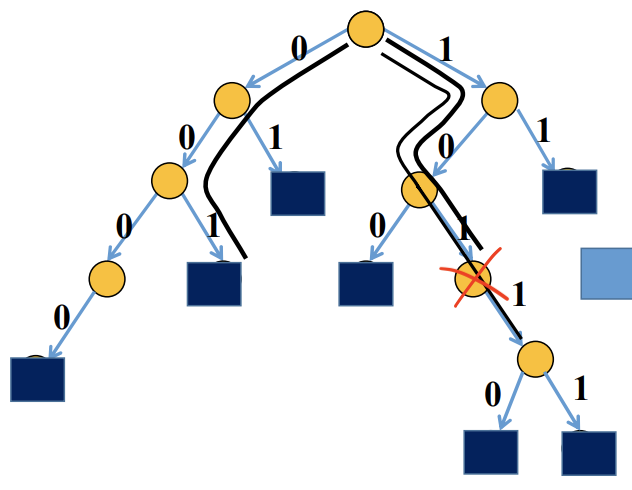
\includegraphics[height=3.4cm,width=0.6\linewidth]{images/prefix-encoding.png} 
    \item for each prefix code $A$ of $n$ alphabets, there exists a binary tree $T$ on $n$ leaves s.t. there is a \textbf{bijective mapping} between the alphabets and the leaves
    \item $OPT_{ABL}(A) = OPT_{ABL}(A') + f(a_1) + f(a_2)$
    \item $ABL(\gamma) = \sum\limits_{x \in A} f(x) \cdot \vert \gamma(x) \vert = \sum\limits_{x \in A} f(x) \cdot \vert depth_T (x) \vert$
    \item binary tree which is an \textit{optimal} prefix coding must be \textbf{full binary tree}.
      \begin{itemize}[topsep=0pt,noitemsep,wide=0pt, leftmargin=\dimexpr\labelwidth + 2\labelsep\relax]
        \item every internal node has degree exactly 2
        \item multiple possible optimal trees - most optimal depends on alphabet frequencies
      \end{itemize}
    \item accounting for alphabet \textbf{frequencies}:
      \begin{itemize}[topsep=0pt,noitemsep,wide=0pt, leftmargin=\dimexpr\labelwidth + 2\labelsep\relax]
        \item let $a_1, a_2, \dots, a_n$ be alphabets of $A$ in non-decreasing order of freq.
        \item $a_1$ must be a leaf node; $a_2$ \textit{can} be a sibling of $a_1$
        \item there exists an optimal prefix coding in which $a_1$ and $a_2$ are siblings
      \end{itemize}
    \item derivation of optimal prefix coding: \textbf{Huffman's algorithm}
      \begin{itemize}[topsep=0pt,noitemsep,wide=0pt, leftmargin=\dimexpr\labelwidth + 2\labelsep\relax]
        \item keep merging the two least frequent items to create a new alphabet $a'$
        \item remove $a_1$ $a_2$ and replace with $a'$
      \end{itemize}
  \end{itemize}

  \begin{minipage}[c]{0.65\linewidth}
    \begin{verbatim}

Huffman(C):
  Q = new PriorityQueue(C)
  while Q:
    allocate a new node z
    z.left = x = extractMin(Q)
    z.right = y = extractMin(Q)
    z.val = x.val + y.val
    Q.add(z)
  return extractMin(Q) // root
    \end{verbatim}
  \end{minipage}
  \begin{minipage}[c]{0.32\linewidth}
    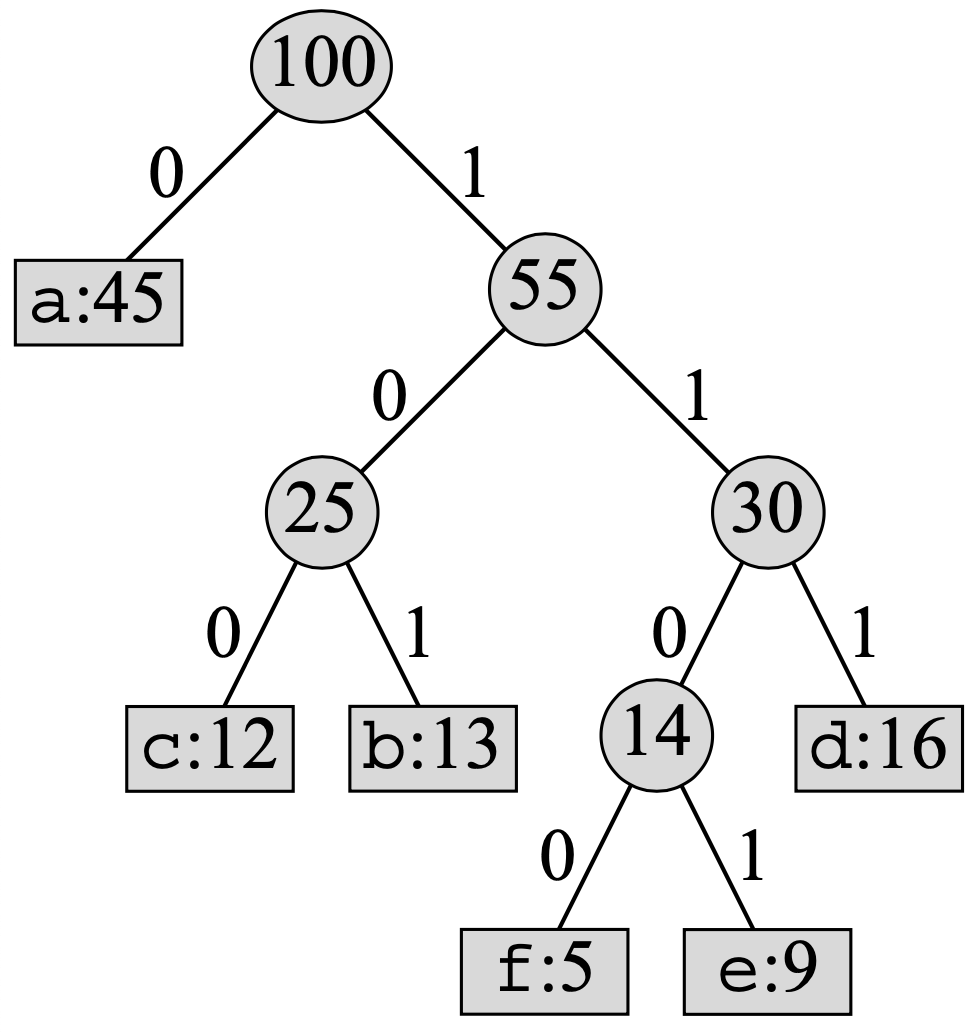
\includegraphics[width=0.95\linewidth]{images/huffman.png} 
  \end{minipage}


\subsection*{08. Amortized Analysis}

\begin{itemize}[topsep=0pt,noitemsep,wide=0pt, leftmargin=\dimexpr\labelwidth + 2\labelsep\relax]
  \item \definition{amortized analysis} guarantees the \textit{average} performance of each operation in the \textit{worst case}.
  \item total amortized cost provides an \textit{upper bound} on the total true cost
  \item For a sequence of $n$ operations $o_1, o_2, \dots, o_n$, 
    \begin{itemize}[topsep=0pt,noitemsep,wide=0pt, leftmargin=\dimexpr\labelwidth + 2\labelsep\relax]
      \item let $t(i)$ be the time complexity of the $i$-th operation $o_i$
      \item let $f(n)$ be the \textit{worst-case} time complexity for \textit{any} of the $n$ operations
      \item let $T(n)$ be the time complexity of all $n$ operations
    \end{itemize}
\end{itemize}

\begin{tightcenter}
  $T(n) = \sum^n_{i=1} t(i) = n f(n)$
\end{tightcenter}

\subsubsection{Types of Amortized Analysis}

\subsubsubsection{Aggregate method}

\begin{itemize}[topsep=0pt,noitemsep,wide=0pt, leftmargin=\dimexpr\labelwidth + 2\labelsep\relax]
  \item look at the whole sequence, sum up the cost of operations and take the average - simpler but less precise
  \item e.g. binary counter - amortized $O(1)$ 
  \item e.g. queues (with \texttt{INSERT} and \texttt{EMPTY}) - amortized $O(1)$
\end{itemize}

\subsubsubsection{Accounting method}

\begin{itemize}[topsep=0pt,noitemsep,wide=0pt, leftmargin=\dimexpr\labelwidth + 2\labelsep\relax]
  \item charge the $i$-th operation a fictitious amortized cost $c(i)$ 
    \begin{itemize}[topsep=0pt,noitemsep,wide=0pt, leftmargin=\dimexpr\labelwidth + 2\labelsep\relax]
      \item \textbf{amortized cost} $c(i)$ is a fixed cost for each operation
      \item \textbf{true cost} $t(i)$ depends on when the operation is called
    \end{itemize}
  \item amortized cost $c(i)$ must satisfy:
    \begin{tightcenter}
      $\sum^n_{i=1} t(i) \leq \sum^n_{i=1} c(i) $ for all $n$
    \end{tightcenter}
  \item take the extra amount for cheap operations early on as "credit" paid in advance for expensive operations
    \begin{itemize}[topsep=0pt,noitemsep,wide=0pt, leftmargin=\dimexpr\labelwidth + 2\labelsep\relax]
      \item \textbf{invariant}: bank balance never drops below 0
    \end{itemize}
  \item the total amortized cost provides an \textbf{upper bound} on the total true cost
\end{itemize}

\subsubsubsection{Potential method}

\begin{itemize}[topsep=0pt,noitemsep,wide=0pt, leftmargin=\dimexpr\labelwidth + 2\labelsep\relax]
  \item $\phi$ : potential function associated with the algo/DS
  \item $\phi(i)$: potential at the end of the $i $-th operation
  \item $c_i$ : amortized cost of the $i$-th operation
  \item $t_i$ : true cost of the $i$-th operation
    \begin{tightcenter}
      $c_i = t_i + \phi(i) - \phi(i-1)$ 

      $\sum^n_{i=1} c_i = \phi(n) - \phi(0) + \sum^n_{i=1} t_i$
    \end{tightcenter}
  \item hence as long as $\phi(n) \geq 0$, then amortized cost is an upper bound of the true cost. Generally in \underline{expensive operation}, we want to see if there is a quantity \textit{decreasing} during this operation
    \begin{tightcenter}
      $\sum^n_{i=1} c_i \geq \sum^n_{i=1} t_i$
    \end{tightcenter}
  \item usually take $\phi(0) = 0$
  \item \textbf{e.g.} for queue:
    \begin{itemize}[topsep=0pt,noitemsep,wide=0pt, leftmargin=\dimexpr\labelwidth + 2\labelsep\relax]
      \item let $\phi(i)$ = \# of elements in queue after the $i$-th operation
      \item amortized cost for insert: $c_i = t_i + \phi(i) - \phi(i-1) = 1 + 1 = 2$
      \item amortized cost for empty (for $k$ elements): $c_i = t_i + \phi(i) - \phi(i-1) = k + 0 - k = 0 $
    \end{itemize}
  \item try to keep $c(i)$ small: using $c(i) = t(i) + \Delta \phi_i$
    \begin{itemize}[topsep=0pt,noitemsep,wide=0pt, leftmargin=\dimexpr\labelwidth + 2\labelsep\relax]
      \item if $t(i)$ is small, we want $\Delta \phi_i$ to be positive and small
      \item if $t(i)$ is large, we want $\Delta \phi_i$ to be negative and large 
    \end{itemize}
\end{itemize}

\subsubsubsection{e.g. Dynamic Table (insertion only)}

\textbf{Aggregate method}

\begin{tightcenter}
  cost of $n$ insertions = $\sum^n_{i=1} t(i) \leq n + \sum^{ \lfloor \log(n-1) \rfloor  }_{j=1} 2^j \leq 3n$
  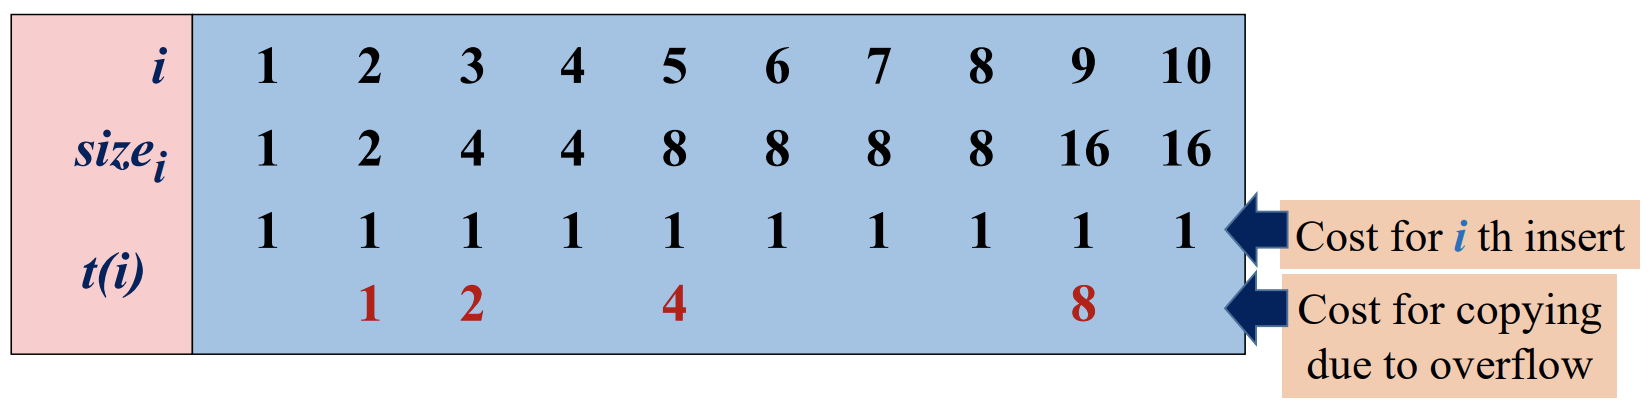
\includegraphics[width=0.95\linewidth]{images/aggregate.png} 
\end{tightcenter}

\textbf{Accounting method}

\begin{itemize}[topsep=0pt,noitemsep,wide=0pt, leftmargin=\dimexpr\labelwidth + 2\labelsep\relax]
  \item charge \$3 per insertion
    \begin{itemize}[topsep=0pt,noitemsep,wide=0pt, leftmargin=\dimexpr\labelwidth + 2\labelsep\relax]
      \item \$1 for insertion itself
      \item \$1 for moving itself when the table expands
      \item \$1 for moving one of the existing items when the table expands
    \end{itemize}
\end{itemize}

\textbf{Potential method}

\begin{tightcenter}
  let $\phi(i) = 2i - size(T)$
  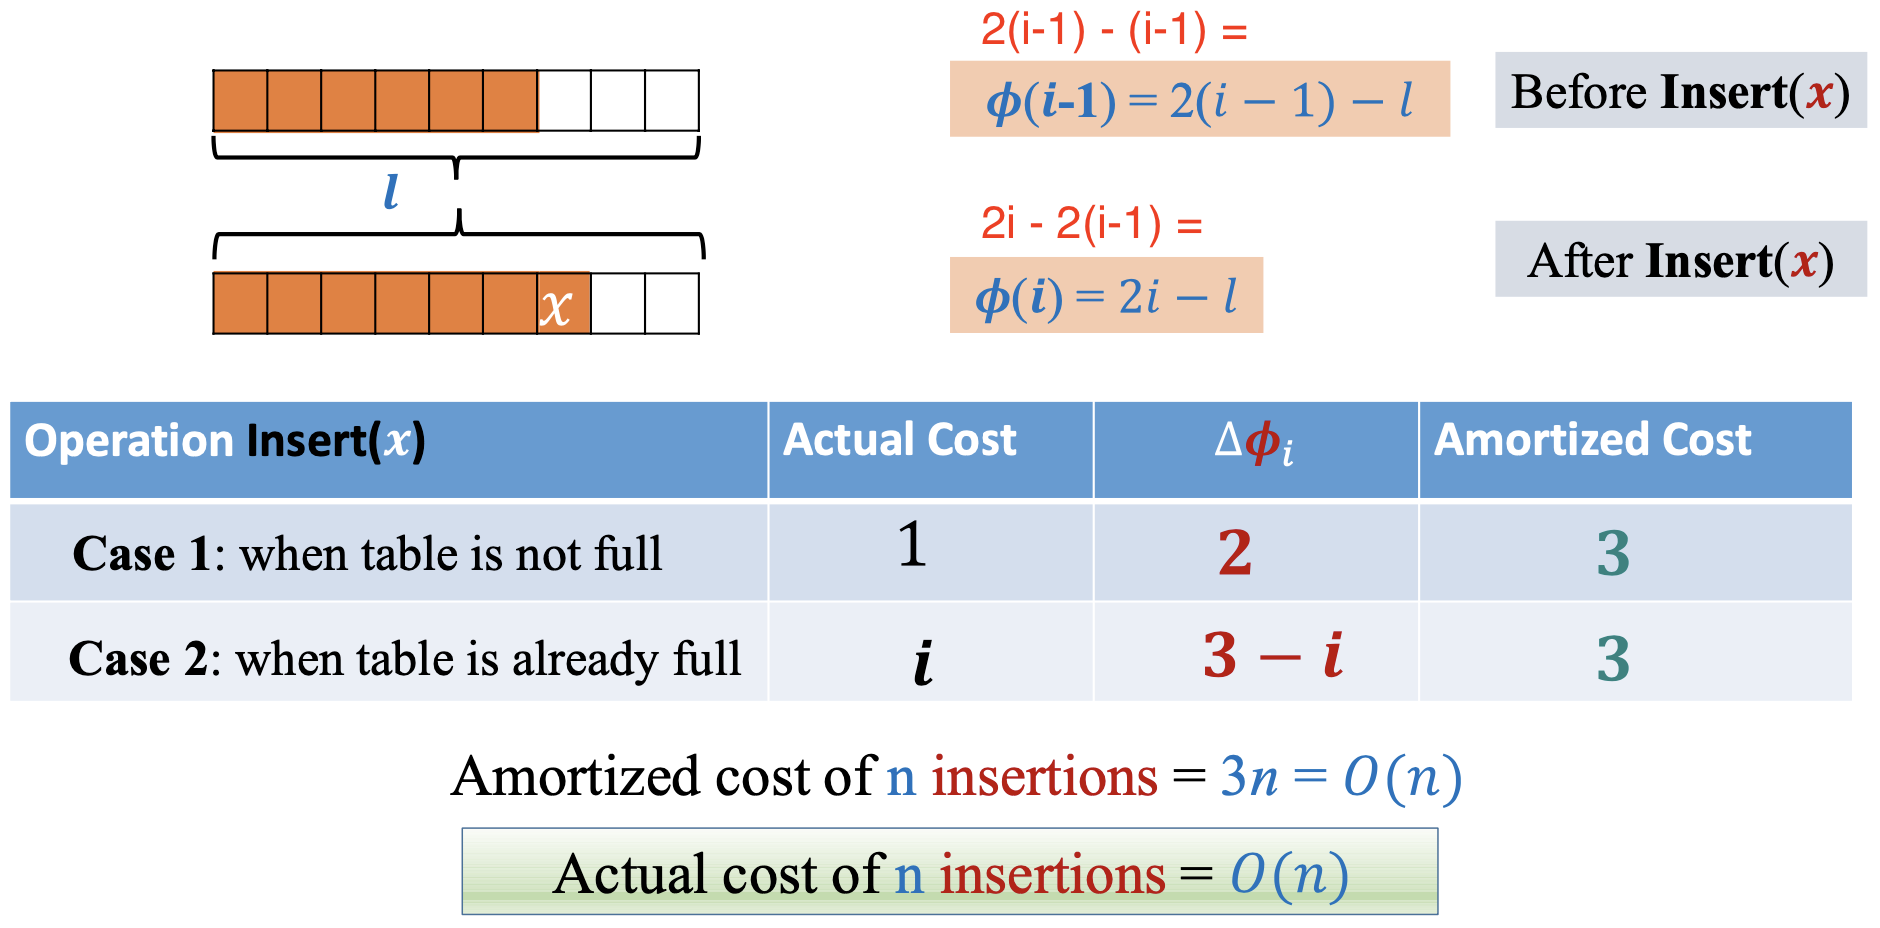
\includegraphics[width=0.95\linewidth]{images/potential.png} 
\end{tightcenter}

\begin{itemize}[topsep=0pt,noitemsep,wide=0pt, leftmargin=\dimexpr\labelwidth + 2\labelsep\relax]
  \item show that SUM of amortized cost $\geq$ SUM of actual cost
  \item conclude that sum of amortized cost is $O(f(n)) \Rightarrow$ sum of actual cost is $O(f(n))$
\end{itemize}


\subsection{9. REDUCTIONS \& INTRACTABILITY}

\subsubsection{Reduction}

Consider two problems $A$ and $B$, $A$ can be solved as follows:

\begin{enumerate}[topsep=0pt,noitemsep,wide=0pt, leftmargin=\dimexpr\labelwidth + 2\labelsep\relax]
  \item convert instance $\alpha$ of $A$ to an instance of $\beta$ in $B$
  \item solve $\beta$ to obtain a solution
  \item based on the solution of $\beta$, obtain the solution of $\alpha$.
  \item $\Rightarrow$ then we say $A$ \textbf{reduces} $B$.
\end{enumerate}

\begin{tightcenter}
  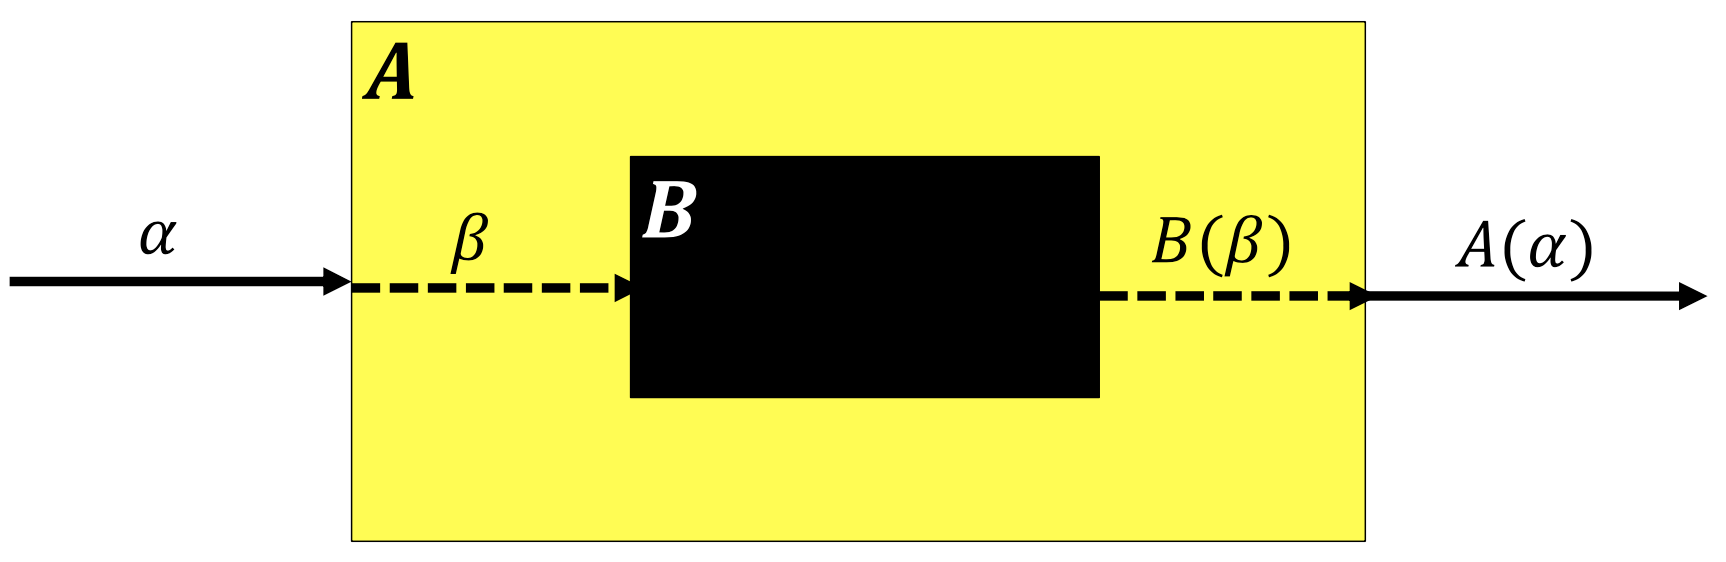
\includegraphics[width=0.7\linewidth]{images/cs3230-reduction-AB.png} 
\end{tightcenter}

\definition{instance} another word for input

\subsubsubsection{e.g. Matrix Multiplication \& Squaring}

\begin{itemize}[topsep=0pt,noitemsep,wide=0pt, leftmargin=\dimexpr\labelwidth + 2\labelsep\relax]
  \item \textsc{Mat-Multi}: matrix multiplication
    \begin{itemize}[topsep=0pt,noitemsep,wide=0pt, leftmargin=\dimexpr\labelwidth + 2\labelsep\relax]
      \item \textit{input}: two $N \times N$ matrices  $A$ and $B$.
      \item \textit{output}: $A \times B$
    \end{itemize}
  \item \textsc{Mat-Sqr}: matrix squaring
    \begin{itemize}[topsep=0pt,noitemsep,wide=0pt, leftmargin=\dimexpr\labelwidth + 2\labelsep\relax]
      \item \textit{input}: one $N \times N$ matrix $C$. \textit{output}: $C \times C$
    \end{itemize}
  \item \textsc{Mat-Sqr} can be reduced to \textsc{Mat-Multi}
    \begin{itemize}[topsep=0pt,noitemsep,wide=0pt, leftmargin=\dimexpr\labelwidth + 2\labelsep\relax]
      \item \textit{Proof}. Given input matrix $C$ for \textsc{Mat-Sqr}, let $A=C$ and  $B=C$ be inputs for \textsc{Mat-Multi}. Then $AB=C^2$.
    \end{itemize}
  \item \textsc{Mat-Multi} can also be reduced to \textsc{Mat-Sqr}!
    \begin{itemize}[topsep=0pt,noitemsep,wide=0pt, leftmargin=\dimexpr\labelwidth + 2\labelsep\relax]
      \item \textit{Proof}. let $C = \left[ \begin{smallmatrix} 0 & A \\ B & 0 \end{smallmatrix} \right]$
        $\Rightarrow C^2 = \left[\begin{smallmatrix} 0 & A \\ B & 0 \end{smallmatrix}\right] \left[\begin{smallmatrix} 0 & A \\ B & 0 \end{smallmatrix}\right] = \left[ \begin{smallmatrix} AB & 0 \\ 0 & BA \end{smallmatrix} \right] $
    \end{itemize}
\end{itemize}

\subsubsubsection{T-Sum}

\begin{itemize}[topsep=0pt,noitemsep,wide=0pt, leftmargin=\dimexpr\labelwidth + 2\labelsep\relax]
  \item \textsc{0-Sum}: given array $A$, output $i, j \in (1, n)$ such that $A[i] + A[j] = 0$
  \item \textsc{T-Sum}: given array $B$, output $i, j \in (1, n)$ such that $B[i] + B[j] = T$
  \item \textbf{reduce \textsc{T-Sum} to \textsc{0-Sum}}:
    \begin{itemize}[topsep=0pt,noitemsep,wide=0pt, leftmargin=\dimexpr\labelwidth + 2\labelsep\relax]
      \item given array $B$, define array  $A$ s.t. $A[i] = B[i] - T/2$.
      \item if $i, j$ satisfy $A[i] + A[j] = 0$, then $B[i] + B[j] = T$.
    \end{itemize}
\end{itemize}

\subsubsubsection{$p(n)$-time Reduction}

\begin{itemize}[topsep=0pt,noitemsep,wide=0pt, leftmargin=\dimexpr\labelwidth + 2\labelsep\relax]
  \item \definition{$p(n)$-time Reduction} if for any instance $\alpha$ of problem $A$ of size $n$, 
    \begin{itemize}[topsep=0pt,noitemsep,wide=0pt, leftmargin=\dimexpr\labelwidth + 2\labelsep\relax]
      \item an instance $\beta$ for $B$ can be constructed in $p(n)$ time
      \item a solution to problem $A$ for input $\alpha$ can be recovered from a solution to problem $B$ for input $\beta$ in time $p(n)$.
    \end{itemize}
  \item \hl{$n$ is in \textbf{bits}!}
  \item if there is a $p(n)$-time reduction from problem $A$ to $B$ and a $T(n)$-time algorithm to solve problem $B$, then there is a $T(O(p(n))) + O(p(n))$ time algorithm to solve $A$.
\end{itemize}

\begin{tightcenter}
  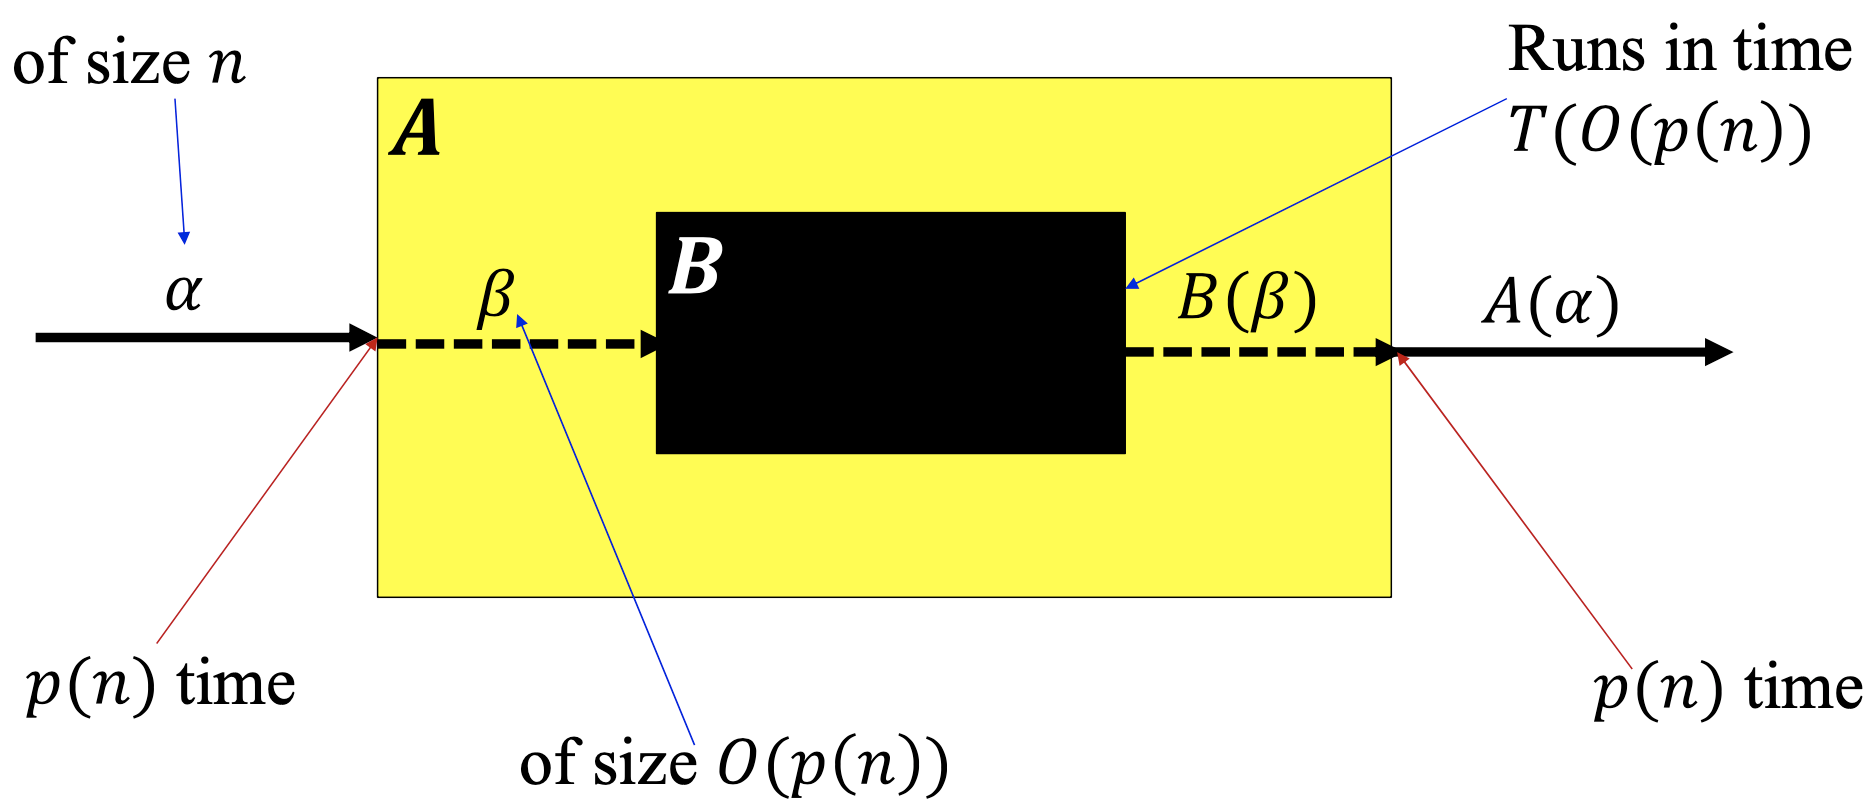
\includegraphics[width=0.8\linewidth]{images/cs3230-reduction-pn.png} 
\end{tightcenter}

\begin{itemize}[topsep=0pt,noitemsep,wide=0pt, leftmargin=\dimexpr\labelwidth + 2\labelsep\relax]
  \item \definition{$A \leq_P B$} if there is a $p(n)$-time reduction from $A$ to $B$ for some polynomial function $p(n) = O(n^c)$ for some constant $c$. ("$A$ is a special case of $B$")
    \begin{itemize}[topsep=0pt,noitemsep,wide=0pt, leftmargin=\dimexpr\labelwidth + 2\labelsep\relax]
      \item if $B$ has a polynomial time algorithm, then so does $A$
      \item "polynomial time" $\approx$ reasonably efficient
    \end{itemize}
  \item $A \leq_P B, B \leq_P C \Rightarrow A \leq_P C$
\end{itemize}

\subsubsection{Polynomial Time}

\begin{itemize}[topsep=0pt,noitemsep,wide=0pt, leftmargin=\dimexpr\labelwidth + 2\labelsep\relax]
  \item \definition{polynomial time} runtime is polynomial in the \textbf{length of the encoding} of the problem instance
  \item \ildefinition{"standard" encodings} 
    \begin{itemize}[topsep=0pt,noitemsep,wide=0pt, leftmargin=\dimexpr\labelwidth + 2\labelsep\relax]
      \item binary encoding of integers
      \item list of parameters enclosed in braces (graphs/matrices)
    \end{itemize}
  \item \definition[algorithm]{pseudo-polynomial} runs in time polynomial in the \textbf{numeric value} if the input but is \textbf{exponential} in the \textbf{length} of the input
    \begin{itemize}[topsep=0pt,noitemsep,wide=0pt, leftmargin=\dimexpr\labelwidth + 2\labelsep\relax]
      \item e.g. DP algo for \textsc{Knapsack} since $W$ is in numeric value
    \end{itemize}
  \item \textsc{Knapsack} is NOT polynomial time: $O(nW \log M)$ but $W$ is not the number of bits
  \item \textsc{Fractional Knapsack} is polynomial time: $O(n \log n \log W \log M)$
\end{itemize}


\subsubsection{Decision Problems}

\begin{itemize}[topsep=0pt,noitemsep,wide=0pt, leftmargin=\dimexpr\labelwidth + 2\labelsep\relax]
  \item \definition{decision problem} a function that maps an instance space $I$ to the solution set $\{YES, NO\}$
  \item decision vs optimisation problem:
    \begin{itemize}[topsep=0pt,noitemsep,wide=0pt, leftmargin=\dimexpr\labelwidth + 2\labelsep\relax]
      \item \textbf{decision problem}: given a directed graph $G$, \textit{is there} a path from vertex $u$ to $v$ of length $\leq k$?
      \item \textbf{optimisation problem}: given ..., what is \textit{length} of the shortest path ... ?
      \item convert from \textbf{decision $\rightarrow$ optimisation}: given an instance of the optimisation problem and a number $k$, is there a solution with value $\leq k$?
    \end{itemize}
  \item the decision problem is \textit{no harder than} the optimisation problem.
    \begin{itemize}[topsep=0pt,noitemsep,wide=0pt, leftmargin=\dimexpr\labelwidth + 2\labelsep\relax]
      \item given the optimal solution, check that it is $\leq k$.
      \item if we cannot solve the decision problem quickly $\Rightarrow$ then we cannot solve the optimisation problem quickly
    \end{itemize}
  \item decision $\leq_P$ optimisation
\end{itemize}

\subsubsection{Reductions between Decision Problems}

\textbf{Karp reduction:} given two decision problems $A$ and $B$, a polynomial-time reduction from $A$ to $B$ denoted $A \leq_P B$ is a \ildefinition{transformation} from instances $\alpha$ of $A$ and $\beta$ of $B$ such that
\begin{enumerate}[topsep=0pt,noitemsep,wide=0pt, leftmargin=\dimexpr\labelwidth + 2\labelsep\relax]
  \item $\alpha$ is a \textit{YES}-instance of $A$ $\iff (iff)$ $\beta$ is a \textit{YES}-instance of $B$
  \item the transformation takes polynomial time in the size of $\alpha$
\end{enumerate}

\begin{tightcenter}
  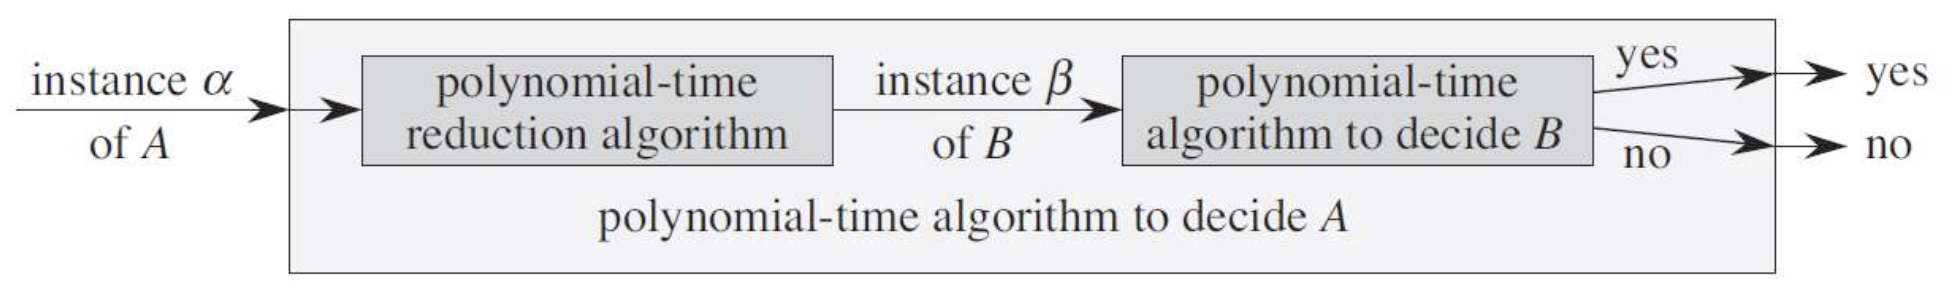
\includegraphics[width=0.95\linewidth]{images/cs3230-reductions-decision-problems.png} 
\end{tightcenter}

\subsubsubsection{Examples}

\begin{itemize}[topsep=0pt,noitemsep,wide=0pt, leftmargin=\dimexpr\labelwidth + 2\labelsep\relax]
  \item \textsc{Independent-Set}: given a graph $G = (V, E)$ and an integer $k$, is there a subset of $\leq k$ vertices such that no 2 are adjacent?
  \item \textsc{Vertex-Cover}: given a graph $G = (V, E)$ and an integer $k$, is there a subset of $\leq k$ vertices such that each edge is incident to \textit{at least one} vertex in this subset?
  \item \textsc{Independent-Set} $\leq_P$ \textsc{Vertex-Cover}
    \begin{itemize}[topsep=0pt,noitemsep,wide=0pt, leftmargin=\dimexpr\labelwidth + 2\labelsep\relax]
      \item \textit{Reduction}: to check whether $G$ has an independent set of size $k$, we check whether $G$ has vertex cover of size $n-k$.
    \end{itemize}
\end{itemize}

\begin{niceproof}
  If \textsc{Independent-Set}, then \textsc{Vertex-Cover}.

  Suppose $(G, k)$ is a \textit{YES}-instance of \textsc{Indep-Set}. Then there is subset $S$ of size $\geq k$ that is an independent set.

  $V-S$ is a vertex cover of size $\leq n-k$. Proof: Let $(u, v) \in E$. Then $u \not\in S$ or $v \not\in S$. 

  So either $u$ or $v$ is in $V-S$, the vertex cover.
\end{niceproof}
\begin{niceproof}
  If \textsc{Vertex-Cover}, then \textsc{Independent-Set}.

  Same as above, but flip IS and VC
\end{niceproof}


\subsubsubsection{e.g. \textsc{Set-Cover}}

Given integers $k$ and $n$, and collection $\mathcal{S}$ of subsets of $\{1, \dots, n\}$, are there $\leq k$ of these subsets whose union equals $\{1, \dots, n\}$?

Claim: \textbf{\textsc{Vertex-Cover} $\leq_P$ \textsc{Set-Cover}}

\textit{Reduction}: given $(G, k)$ instance of \textsc{Vertex-Cover}, generate an instance $(n, k', \mathcal{S})$ of \textsc{Set-Cover}.

\begin{niceproof}
  For each node $v$ in $G$, construct a set $S_v$ containing all its outgoing edges. (Number each edge)
  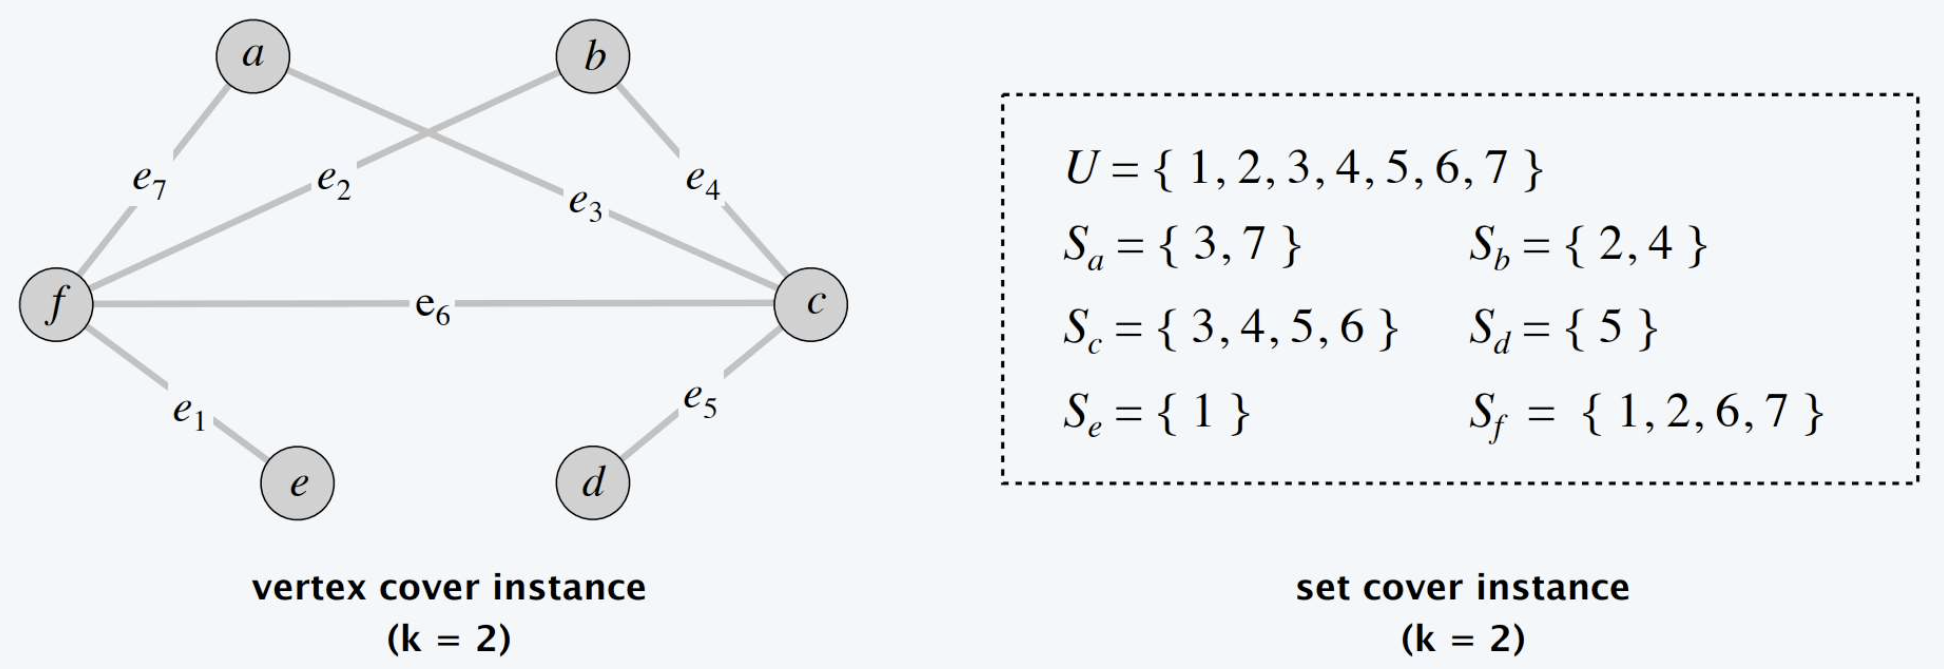
\includegraphics[width=0.95\linewidth]{images/cs3230-vertex-reduce-to-set-cover.png} 
\end{niceproof}


\subsubsubsection{e.g. 3-SAT}

  \begin{itemize}
    \item \textbf{SAT}: given a CNF formula $\Phi$, does it have a satisfying truth assignment?
      \begin{itemize}[topsep=0pt,noitemsep,wide=0pt, leftmargin=\dimexpr\labelwidth + 2\labelsep\relax]
        \item literal: a boolean variable or its negation $x, \bar{x}$
        \item clause: a disjunction (OR) of literals
        \item conjunctive normal form (CNF): formula $\Phi$ that is a conjunction (AND) of clauses
      \end{itemize}
    \item \definition{3-SAT} SAT where each clause contains exactly $3$ literals
    \item \textbf{3-SAT $\leq_P$ \textsc{Independent-Set}}
      \begin{itemize}[topsep=0pt,noitemsep,wide=0pt, leftmargin=\dimexpr\labelwidth + 2\labelsep\relax]
        \item \textit{Reduction}: Construct an instance $(G, k)$ of \textsc{Indep-Set} s.t. $G$ has an independent set of size $k \iff \Phi$ is satisfiable
          \begin{itemize}[topsep=0pt,noitemsep,wide=0pt, leftmargin=\dimexpr\labelwidth + 2\labelsep\relax]
            \item node: each literal term
            \item edge: connect 3 literals in a clause in a triangle
            \item edge: connect literal to all its negations
            \item reduction runs in polynomial time
          \end{itemize}
        \item $\Rightarrow$ for $k$ clauses, connecting $k$ vertices form an independent set in $G$. 
      \end{itemize}
      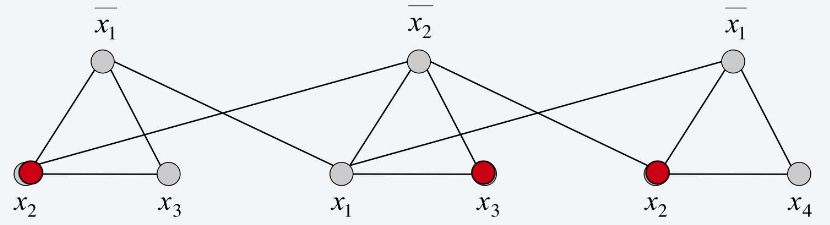
\includegraphics[width=0.95\linewidth]{images/3sat.png} 
  \end{itemize}

\subsection{10. NP-COMPLETENESS}

  \begin{itemize}[topsep=0pt,noitemsep,wide=0pt, leftmargin=\dimexpr\labelwidth + 2\labelsep\relax]
    \item \definition{P} the class of \textit{decision} problems solvable in (deterministic) polynomial time
    \item \definition{NP} the class of \textit{decision} problems for which polynomial-time verifiable \textbf{certificates} of YES-instances exist.
      \begin{itemize}[topsep=0pt,noitemsep,wide=0pt, leftmargin=\dimexpr\labelwidth + 2\labelsep\relax]
        \item aka \textit{non-deterministic polynomial}
        \item i.e. no poly-time algo, but verification can be poly-time
        \item \definition{certificate} result that can be checked in poly-time to verify correctness
      \end{itemize}
    \item $P \subseteq NP$: any problem in \textbf{P} is in \textbf{NP}.
      \begin{itemize}[topsep=0pt,noitemsep,wide=0pt, leftmargin=\dimexpr\labelwidth + 2\labelsep\relax]
        \item if $P=NP$, then all these algos can be solved in poly time
      \end{itemize}
  \end{itemize}

  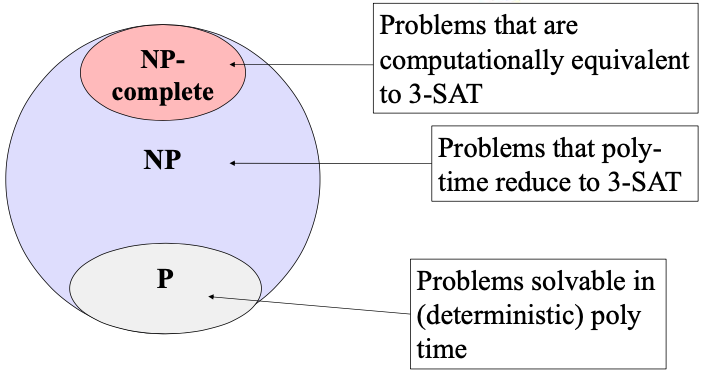
\includegraphics[width=0.95\linewidth]{images/pequalnp.png} 

  \subsubsection{NP-Hard and NP-Complete}

  \begin{itemize}[topsep=0pt,noitemsep,wide=0pt, leftmargin=\dimexpr\labelwidth + 2\labelsep\relax]
    \item a problem $A$ is said to be \ildefinition{NP-Hard} if for \textit{every} problem $B \in NP$, $B \leq_P A$.
      \begin{itemize}[topsep=0pt,noitemsep,wide=0pt, leftmargin=\dimexpr\labelwidth + 2\labelsep\relax]
        \item aka $A$ is at least as hard as every problem in \textbf{NP}.
      \end{itemize}
    \item a problem $A$ is said to be \ildefinition{NP-Complete} if it is in \textbf{NP} and is also \textbf{NP-Hard}
      \begin{itemize}[topsep=0pt,noitemsep,wide=0pt, leftmargin=\dimexpr\labelwidth + 2\labelsep\relax]
        \item aka the hardest problems in NP.
      \end{itemize}
    \item \definition{Cook-Levin Theorem} every problem in NP-Hard can be poly-time \textit{reduced} to 3-SAT. Hence, \textbf{3-SAT is NP-Hard and NP-Complete}.
    \item NP-Complete problems can still be approximated in poly-time! (e.g. greedy algorithm gives a 2-approximation for \textsc{Vertex-Cover})
  \end{itemize}

  \subsubsection{showing NP-Completeness}

  \begin{enumerate}[topsep=0pt,noitemsep,wide=0pt, leftmargin=\dimexpr\labelwidth + 2\labelsep\relax]
    \item show that $X$ is in NP. $\Rightarrow$ a YES-instance has a certificate that can be verified in polynomial time
    \item show that $X$ is NP-hard
      \begin{itemize}[topsep=0pt,noitemsep,wide=0pt, leftmargin=\dimexpr\labelwidth + 2\labelsep\relax]
        \item by giving a poly-time reduction from another NP-hard problem $A$ to $X$.
          $\quad \Rightarrow$ $X$ is at least as hard as $A$
        \item reduction should \textit{not} depend on whether the instance of $A$ is a YES- or NO-instance
      \end{itemize}
    \item show that the reduction is valid
      \begin{enumerate}[topsep=0pt,noitemsep,wide=0pt, leftmargin=\dimexpr\labelwidth + 2\labelsep\relax]
        \item reduction runs in poly time
        \item if the instance of $A$ is a YES-instance, then the instance of $X$ is also a YES-instance
        \item if the instance of $A$ is a NO-instance, then the instance of $X$ is also a NO-instance
      \end{enumerate}
  \end{enumerate}

  \begin{tightcenter}
    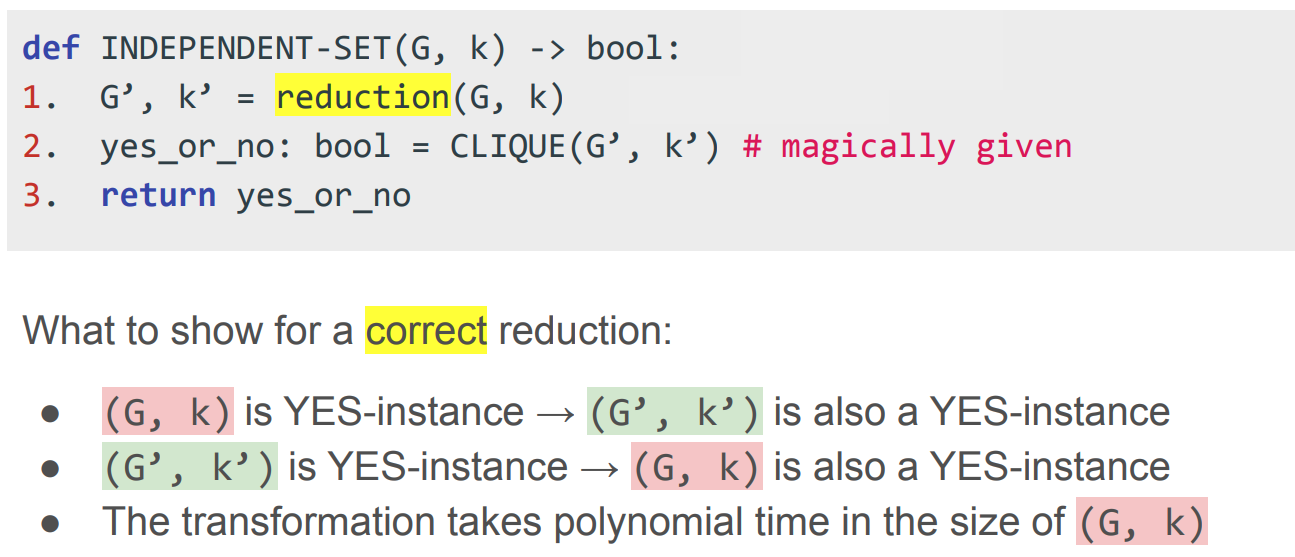
\includegraphics[width=0.98\linewidth]{images/shownpcomplete.png} 
  \end{tightcenter}

  \subsubsection{showing NP-HARD}

  \begin{enumerate}[topsep=0pt,noitemsep,wide=0pt, leftmargin=\dimexpr\labelwidth + 2\labelsep\relax]
    \item take any \textbf{NP-Complete} problem $A$ 
    \item show that $A \leq_P X$
  \end{enumerate}

  \subsection{11. Linear Time Sorting and Selection}
  \subsubsubsection{Direct Addressing Table}
  \begin{lstlisting}
C = [0]*(k+1) # create the frequency DAT [0..k], O(k)
for Ai in A: # O(n), at the end, C[i] = frequency of i
  C[Ai] += 1
for i in range(k+1): # O(k+n)
  print(*[i] * C[i], end=’ ’) # set format yourself
  \end{lstlisting}
  \begin{itemize}[topsep=0pt,noitemsep,wide=0pt, leftmargin=\dimexpr\labelwidth + 2\labelsep\relax]
    \item No comparisons between element $\rightarrow$ not comparison based sorting
    \item Trade-off \textit{memory} (DAT) to break $\Omega(n\log n)$ lower bound
    \item If $k \in O(n)$ then $O(n + k)$ counting sort takes $O(n)$ time
    \item It requires \textbf{big memory} for the frequency counter DAT C. $\Rightarrow$ If k is big, we may not be able to create a DAT C to cover [0..k]
    \item We want to set k big enough (vs the available working memory), but not too big that we cannot even run the algorithm.
  \end{itemize}

  \subsubsubsection{Counting Sort Stable Version}
  \begin{lstlisting}
C = [0]*(k+1) # create the frequency DAT [0..k], O(k)
for Ai in A: # O(n), at the end, C[i] = freq. of i
  C[Ai] += 1
for i in range(1, k+1): # O(k), C[i] = num ints <= i
  C[i] += C[i-1] # aka the ’prefix sum’
  B = [0] * n # output (sorted) array
for i in range(n-1, -1, -1): # O(n), from B2F
  C[A[i]] -= 1 # decrease first (0-based indexing)
  B[C[A[i]]] = A[i] # A[i] is placed at C[A[i]] in B
print(*B) # B is the sorted version of A, and stable
\end{lstlisting}

\subsubsubsection{Radix Sort - Iterated Counting Sort}
\begin{lstlisting}
for i <- 1 to d # note: LSD is from right to left
  sort by the i-th LSD #(using stable Counting Sort)
\end{lstlisting}
\begin{itemize}[topsep=0pt,noitemsep,wide=0pt, leftmargin=\dimexpr\labelwidth + 2\labelsep\relax]
  \item We can use \textbf{proof by induction}: When we have sorted the $i^{th}$ LSD, then the integers are sorted according to their values on the $i^{th}$ LSD.
  \item $P(1)$ holds, as Radix Sort first pass will correctly sort the LSD (we are sure the stable Counting Sort sub-routine is correct).
  \item Suppose $P(i - 1)$ holds, we can show $P(i)$ holds too:
  \begin{itemize}[topsep=0pt,noitemsep,wide=0pt, leftmargin=\dimexpr\labelwidth + 2\labelsep\relax]
    \item The integers are sorted based on the $i^{th}$ LSD on the $i^{th}$ pass.
    \item Now, due to the stable sort subroutine used, within the group of integers that have the same $i^{th}$ LSD, the stable sort algorithm does not change their relative position! $\Rightarrow$ Thus, these integers are correctly sorted!
  \end{itemize}
\end{itemize}

\subsubsubsection{Radix Sort - Analysis}
\begin{itemize}[topsep=0pt,noitemsep,wide=0pt, leftmargin=\dimexpr\labelwidth + 2\labelsep\relax]
  \item If we have $d$ digits, Radix Sort runs $d$ iterations of $O(n + k)$ Counting Sort, thus the overall time complexity in $O(d \cdot (n + k))$.
  \item Setting $k = 10$ (digit $[0..9]$, or base $10$/Decimal), is often \textbf{not} the best setup.
  \item If $b$-bit word is broken in to $\frac{b}{r}$ groups of $r$-bit words:
  \begin{itemize}[topsep=0pt,noitemsep,wide=0pt, leftmargin=\dimexpr\labelwidth + 2\labelsep\relax]
    \item There are only $d = \frac{b}{r}$ passes now
    \item Each pass takes $O(n+2^r)$ as $k=2^r$
    \item Total time is thus $O(\frac{b}{r}(n+2^r))$, choose $r$ to minimize $O(\frac{b}{r}(n+2^r))$
    \item Optimal $r \approx \log_2 n$ so that $(n+2^r)$ balances
    \item Total time is thus $O(\frac{b}{\log_2 n} \cdot (n + 2^{\log_2 n}))  = O(\frac{b \cdot n}{\log_2 n})$
    \item Now if the integers are in the range of $[0..n^d]$, then $b=\log_2 n^d$ bits or $b=d \cdot \log_2 n$ bits
    \item Thus Radix Sort runs in time $O(\frac{d \cdot \log_2 n \cdot n}{\log_2 n}) = O(d \cdot n)$ | linear time
  \end{itemize}
\end{itemize}

  \subsubsubsection{Quickselect - Pseudocode}
  \begin{lstlisting}
function QuickSelect(A, l, r, i)
  if l == r, return l
  k = Randomized Partition(A, l, r) // random pivot
  if i == k, then return k // found
  else if i < k, then return QuickSelect(A, l, k-1, i)
  else, then return QuickSelect(A, k+1, r, i)
  \end{lstlisting}
  \begin{itemize}[topsep=0pt,noitemsep,wide=0pt, leftmargin=\dimexpr\labelwidth + 2\labelsep\relax]
    \item Best case for QuickSelect is $O(n)$ i.e. one pass of \verb|Randomized_partition|, we find that pivot has rank $k=i$
    \item If the participants sub-routine is \textit{not randomized}, worst case for QuickSelect is similar to worst case of QuickSort $\rightarrow$ $O(n^2)$
  \end{itemize}

  \subsubsubsection{Worse-case Linear-Time Select - Pseudocode}
  \begin{lstlisting}
function Select(A, n, i)
  # step 1 - Theta(n)
  # divide A into ceil(n/5) groups of 5 elements each
  # find the median of each 5-elements group in O(1)
  # step 2, T(n/5)
  # Let B be ceil(n/5) medians of each groups
  Select(B, |B|, |B|/2)) # find median of medians
  # step 3 - Theta(n)
  k = Partition(A, x) # use this specific pivot x
  # Let A’ / A’’ be elements < x / > x, respectively
  # step 4-5-6, similar as Quickselect - T(7n/10)
  if i == k, then return k # found
  else if i < k, then return Select(A’, k-1, i)
  else, return Select(A’’, n-k, i-k)
  \end{lstlisting}  
  \begin{tightcenter}
    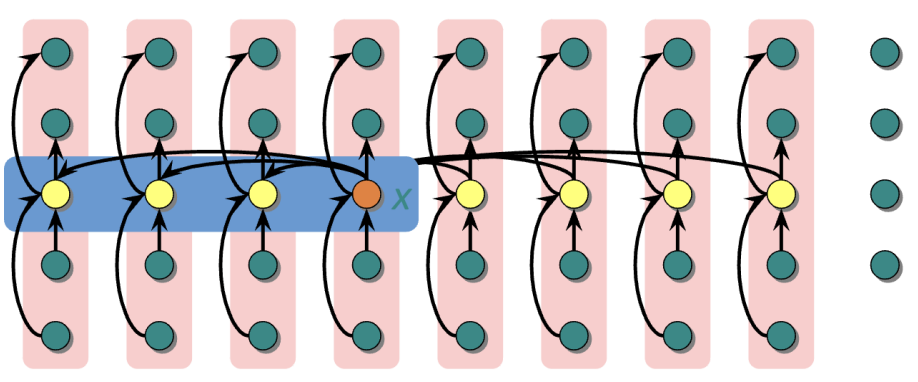
\includegraphics[width=0.98\linewidth]{images/medianofmedians.png} 
  \end{tightcenter}
  \begin{itemize}
    \item Divide the n elements into groups of 5. There are $\lfloor\frac{n}{5}\rfloor$ such groups
    \item Find median of each group in $O(1)$ $\rightarrow$ sort and get index $2$, sorting $5$ elements is $O(1)$, there are $\lfloor\frac{n}{5}\rfloor$ such medians
    \item Recursively Select the median x of the $\lfloor\frac{n}{5}\rfloor$ group medians. This $x$, the \textbf{median of medians}, will be the pivot.
    \item At least half of the group of $5$ medians are $\leq x$, which is at least $\lfloor\lfloor\frac{n}{5}/ 2 \rfloor\rfloor = \lfloor\frac{n}{10}\rfloor$ elements.
    \item $\therefore \geq 3 \cdot \lfloor \frac{n}{10} \rfloor$ elements are $\leq x$ and $\geq x$
    \item For large n, since at least $\lfloor \frac{n}{10} \rfloor$ elements are $leq x$ (or $\geq x$), after partitioning $A$ around $x$, the recursive call to Select (step 5-6) is executed recursively on at most $n - \frac{3n}{10} = \frac{7n}{10}$ elements.
    \item Thus, the recurrence for running time T(n) takes time of not more than $T(n)$  takes time of not more than $T(\frac{n}{5}) + T(\frac{7n}{10}) + \Theta(n)$in the worst case. For small $n$, we can compute $T(n) \in \Theta(1)$.
  \end{itemize}

\subsection{A. Misc. formulas}
\subsubsubsection{A1. Definition of limits}
$\lim_{n\rightarrow\infty}(\frac{f(n)}{g(n)}) = z \Rightarrow$
$\forall \epsilon > 0, \ \exists n_0 > 0, \ \text{s.t.} \ \forall n \geq n_0$:
\framebox{\parbox{\dimexpr\linewidth-67\fboxsep-2\fboxrule}{% 
  $|\frac{f(n)}{g(n)} - z| < \epsilon$
}}

\subsubsubsection{A2. Logarithm/Exponential rules}
\begin{enumerate}[topsep=0pt,noitemsep,wide=0pt, leftmargin=\dimexpr\labelwidth + 2\labelsep\relax]
  \item $\log(M \cdot N) = \log M + \log N \Rightarrow \log(M/N) = \log M - \log N$
  \item $\log(M^k) = k\cdot\log(M) \Rightarrow b^{\log_b(k)} = k$
  \item $\log(1) = 0 \ || \ \log_b(b) = 1 \ || \ \log_b(b^k) = k $ 
\end{enumerate}
\noindent\rule{0.28\textwidth}{0.2pt}
\begin{enumerate}[label=\alph*., topsep=0pt, noitemsep, wide=0pt, leftmargin=\dimexpr\labelwidth + 2\labelsep\relax]
  \item $a^x \times a^y = a^{x+y} \Rightarrow a^x \div a^y = a^{x-y} \ || \ (a^x)^y = a^{x\cdot y}$
  \item For any $a^b$, $a^b = e^{b\ln(a)}$
\end{enumerate}


\subsubsubsection{A3. Helpful approximations}
\begin{enumerate}[topsep=0pt,noitemsep,wide=0pt, leftmargin=\dimexpr\labelwidth + 2\labelsep\relax]
  \item \textbf{stirling's approximation:} 
\begin{itemize}
  \item $T(n) = \sum\limits^n_{i=0} \log (n-i) = \log \prod^n_{i=0} (n-i) = \Theta(n \log n)$ 
  \item OR $n! \approx (\frac{n}{e})^n \sqrt{2\pi n}$
\end{itemize}
  \item \textbf{harmonic number:} \\ $ H_n = \sum\limits_{k=1}^n \frac{1}{k} = \Theta(\lg n) $
  \item \textbf{basel problem:} \\ $\sum\limits^N_{n=1} \frac{1}{n^2} \leq 2 - \frac{1}{N} \xrightarrow{ N \to \infty } 2 $
        $\quad\quad$ because $\sum^N_{n=1} \frac{1}{N^2} \leq 1 + \sum^{\log_3 n}_{x=2} \frac{1}{(x-1)x} = 1 + \sum^N_{n=2} (\frac{1}{n-1} - \frac{1}{n}) = 1 + 1 - \frac{1}{N} = 2 - \frac{1}{N} $
  \item \textbf{number of primes in range:} $\{1, \dots, K\}$ is $> \frac{K}{\ln K} $
  \item \textbf{L'Hôpital's rule:} $\lim_{x \rightarrow c}\frac{f(x)}{g(x)} = \lim_{x \rightarrow c}\frac{f'(x)}{g'(x)}$
\end{enumerate}

\subsubsubsection{A4. Asymptotic bounds}
$1 < \log n < \sqrt{n} < n < n \log n < n^2 < n^3 < 2^n < 2^{2n}$

$\log_a n < n^a < a^n < n^n < n!$

for any $a, b > 0$, $\quad \log_a n < n^b$

\subsubsubsection{A5. Multiple parameters}
for two functions $f(m, n)$ and $g(m,n)$, we say that $f(m, n) = O(g(m, n))$ if there exists constants $c, m_0, n _0$ such that $0 \leq f(m,n) \leq c \cdot g(m,n)$ for all $m \geq m_0$ or $n \geq n_0$.

\subsubsubsection{A6. Example proofs}

\begin{niceproof}
  that $2n^2 = O(n^3)$ 
  \\* let $f(n) = 2n^2$. then $f(n) = 2n^2 \leq n^3$ when $n \geq 2$. 
  \\* set  $c=1$ and $n_0 = 2$.
  \\* we have $f(n) = 2n^2 \leq c \cdot n^3$ for $n \geq n_0$. 
\end{niceproof}

\begin{niceproof}
  $n=o(n^2)$ 

  For any $c>0$, use $n_0 = 2/c$.
\end{niceproof}

\begin{niceproof}
  $n^2 - n =\omega(n)$ 

  For any $c>0$, use $n_0 = 2(c+1)$.
\end{niceproof}

\begin{niceproof}[Example]
  let $f(n) = n$ and $g(n) = n^{1 + \sin (n)}$. 

  Because of the oscillating behaviour of the sine function, there is no $n_0$ for which $f$ dominates $g$ or vice versa.

  Hence, we cannot compare $f$ and $g$ using asymptotic notation.
\end{niceproof}

\begin{niceproof}[Example]
  let $f(n) = n$ and $g(n) = n(2+\sin(n))$.

  Since $\frac{1}{3}g(n) \leq f(n) \leq g(n)$ for all $n \geq 0$, then $f(n) = \Theta(g(n))$.
  (note that limit rules will not work here)
\end{niceproof}

\subsubsubsection{A7. Formulas}
\subsubsubsection{Geometric Series}
\begin{itemize}[topsep=0pt,noitemsep,wide=0pt, leftmargin=\dimexpr\labelwidth + 2\labelsep\relax]
  \item $S_n = \frac{a(1-r^n)}{1-r}$ | $S_\infty = \frac{a}{1-r}$
  \begin{itemize}[topsep=0pt,noitemsep,wide=0pt, leftmargin=\dimexpr\labelwidth + 2\labelsep\relax]
    \item where $a$ is the first term, $r$ is the common ratio, $n$ is number of terms
  \end{itemize}
\end{itemize}
\subsubsubsection{Arithmetic Series}
\begin{itemize}[topsep=0pt,noitemsep,wide=0pt, leftmargin=\dimexpr\labelwidth + 2\labelsep\relax]
  \item $S_n = n (\frac{a_1 + a_n}{2})$, $n$ is number of terms, $a_1$ is first term, $a_n$ is $n^{th}$ term
\end{itemize}
\begin{multicols}{2}
  \subsubsubsection{Ratio Test}
  $L = \lim_{n \to \infty} \frac{a_{n+1}}{a_n}$ 
  \columnbreak
  \[
  \begin{cases}
  L < 1 & \text{\textcolor{red}{\textbf{absolutely convergent}}} \\
  L > 1 \text{ or } L = \infty & \text{\textcolor{purple}{\textbf{divergent}}} \\
  L = 1 & \text{\textcolor{orange}{\textbf{inconclusive}}}
  \end{cases}
  \]
\end{multicols}


\subsection{B. Leetcode pseudo-code}
\subsubsubsection{B1. Coin Change I and II}
\begin{itemize}[topsep=0pt,noitemsep,wide=0pt, leftmargin=\dimexpr\labelwidth + 2\labelsep\relax]
  \item Fewest number of coins needed to make target amount
  \begin{lstlisting}
def coinChange(coins: List[int], amount: int):
  dp = [0] + [float('inf')] * amount
  for coin in coins:
    for target in range(coin, amount + 1):
      dp[target] = min(dp[target], 
                       1 + dp[target - coin])
  if dp[-1] == float('inf'):
    return -1
  else:
    return dp[-1]
  \end{lstlisting}
  \item Number of combinations that make up target amount
  \begin{lstlisting}
def change(amount: int, coins: List[int]):
  dp = [0] * (amount + 1)
  dp[0] = 1
  for coin in coins:
    for target in range(coin, amount + 1):
      dp[target] += dp[target - coin]
  return dp[-1]
  \end{lstlisting}
\end{itemize}
\subsubsubsection{B2. Best time to buy sell stock}
\begin{itemize}[topsep=0pt,noitemsep,wide=0pt, leftmargin=\dimexpr\labelwidth + 2\labelsep\relax]
  \item No cooldown
  \begin{lstlisting}
def maxProfit(self, prices: List[int]) -> int:
  if len(prices) < 2:
    return 0
  l, r = 0, 1
  res = 0
  while r < len(prices):
    profit = prices[r] - prices[l]
    if profit >= 0:
      res = max(res, profit)
    else:
      l = r
    r += 1
  return res
  \end{lstlisting}
  \item With cooldown
  \begin{lstlisting}
def maxProfit(self, prices: List[int]) -> int:
  if not prices:
    return 0
  dp = [[0,0,0] for _ in range(len(prices))]
  # state [buy, sell, cooldown]
  dp[0][0] = -prices[0]
  dp[0][1] = 0
  dp[0][2] = 0
  for i in range(1, len(prices)):
    dp[i][0] = max(dp[i-1][0], dp[i-1][2] 
                      - prices[i])
    dp[i][1] = dp[i-1][0] + prices[i]
    dp[i][2] = max(dp[i-1][1], dp[i-1][2])
  return max(dp[-1][1], dp[-1][2])
  \end{lstlisting}
\end{itemize}

\subsubsubsection{B3. Subsequence}
\begin{itemize}[topsep=0pt,noitemsep,wide=0pt, leftmargin=\dimexpr\labelwidth + 2\labelsep\relax]
  \item Longest \underline{Increasing} subsequence
  \begin{lstlisting}
def lengthOfLIS(self, nums: List[int]) -> int:
  n = len(nums)
  dp = [1] * n
  for i in range(n - 1, -1, -1):
    for j in range(i + 1, n):
      if nums[i] < nums[j]:
        dp[i] = max(dp[i], 1 + dp[j])              
  return max(dp)
  \end{lstlisting}
  \item Longest \underline{Common} subsequence
  \begin{lstlisting}
def longestCommonSubsequence(self, text1: str, text2: str) -> int:
  dp = [[0] * (len(text2) + 1) for _ in range(len(text1) + 1)]
  for i in range(len(text1) - 1, -1, -1):
    for j in range(len(text2) - 1, -1, -1):
      if text1[i] == text2[j]:
        dp[i][j] = 1 + dp[i+1][j+1]
      else:
        dp[i][j] = max(dp[i+1][j], dp[i][j+1])
  return dp[0][0]
  \end{lstlisting}
\end{itemize}

\subsubsubsection{B4. Distinct Subsequence}
If subsequence has last element that is repeated with current element $x_j = x_i$, where $j < i$, there is an additional subsequence that is repeated.
Otherwise, there can be 2 subsequences that end with either $x_j$ or $x_i$.
\begin{lstlisting}
def distinctSubseqII(self, S):
  res, end = 0, collections.Counter()
  for c in S:
    res, end[c] = res * 2 + 1 - end[c], res + 1
  return res
\end{lstlisting}

\subsubsubsection{B5. Jump Game II}
\begin{lstlisting}
def jump(self, nums: List[int]) -> int:
 if len(nums) <= 1: return 0
 l, r = 0, nums[0]
 res = 1
 while r < len(nums) - 1:
  res += 1
  nxt = max(i + nums[i] for i in range(l, r + 1))
  l, r = r, nxt
 return res
\end{lstlisting}

\subsubsubsection{B6. Container with most water}
\begin{lstlisting}
def maxArea(self, height: List[int]) -> int:
 l, r = 0, len(height) - 1
 res = 0
 while l <= r:
  width = r - l
  length = min(height[l], height[r])
  res = max(res, width * length)
  if height[l] < height[r]:
   l += 1
  else:
   r -= 1
 return res
\end{lstlisting}

\subsubsubsection{B7. Maximum subarray}
\begin{lstlisting}
def maxSubArray(self, nums: List[int]) -> int:
  ans, curr = 0, 0
  for i in range(len(nums)):
      if curr < 0:
          curr = 0
      curr += nums[i]
      ans = max(ans, curr)
  return ans
\end{lstlisting}

\subsubsubsection{B8. Gas Station}
\begin{lstlisting}
def canCompleteCircuit(gas: List[int], cost: List[int]) -> int:
  if (sum(gas) - sum(cost) < 0):
      return -1
  gas_tank, start_index = 0, 0
  for i in range(len(gas)):
      gas_tank += gas[i] - cost[i]
      if gas_tank < 0:
          start_index = i+1
          gas_tank = 0
      
  return start_index
\end{lstlisting}

\subsection{C. Recurrences}
\subsubsubsection{C1. $T(n) = 9T(\frac{n}{3}) + n^2/lg n$}
\includegraphics*[width=8.5cm, height=3.8cm]{images/recurrence1.PNG}

\subsubsubsection{C2. $T(2^n) = T(2^{n-1}) + \cdots + T(2^1) + T(2^0)$}
\framebox{\parbox{\dimexpr\linewidth-2\fboxsep-2\fboxrule}{% 
  \begin{enumerate}[topsep=0pt,noitemsep,wide=0pt, leftmargin=\dimexpr\labelwidth + 2\labelsep\relax]
    \item $T(2^n) - T(2^{n-1}) = T(2^{n-1}) + n^2 - (n-1)^2$
    \item $T(2^n) = 2T(2^{n-1}) + 2n - 1 || 2^n = N \Rightarrow N = 2^n \Rightarrow lgN = nlg2 \approx n$
    \item $T(N) = 2T(N/2) + lgN + 1 \Rightarrow$ by M.T, $T(N) = N \Rightarrow T(2^n) = \Theta(2^n)$
  \end{enumerate}
}}

\subsection{D. Greedy Algorithms Proof:}
\subsubsubsection{D1. Scheduling}
\begin{itemize}[topsep=0pt,noitemsep,wide=0pt, leftmargin=\dimexpr\labelwidth + 2\labelsep\relax]
  \item \textbf{Optimal Substructure:}
  \begin{itemize}[topsep=0pt,noitemsep,wide=0pt, leftmargin=\dimexpr\labelwidth + 2\labelsep\relax]
    \item Suppose an optimal scheduling $S$ contains activity $a_j$, let:
    \begin{itemize}[topsep=0pt,noitemsep,wide=0pt, leftmargin=\dimexpr\labelwidth + 2\labelsep\relax]
      \item $Before_j = \{a_i : f_i \leq s_j \}$ (finish before activity $a_j$ starts)
      \item $After_j = \{a_i : s_i \geq f_j \}$ (start after activity $a_j$ finishes)
      \item $\therefore S$ contains optimal scheduling for $Before_j$ and $After_j$
      \item Proof by contradiction
      \begin{itemize}[topsep=0pt,noitemsep,wide=0pt, leftmargin=\dimexpr\labelwidth + 2\labelsep\relax]
        \item Assume $S$ is an optimal schedule for the entire set of activities but does not contain optimal schedules for $Before_j$ or $After_j$
        \item Replace the suboptimal schedule in $S$ with the optimal scheduling for $Before_j$ or $After_j$
        \item $\therefore S$ now has \underline{more} activities, contradicting the assumption that $S$ is optimal
      \end{itemize}
    \end{itemize}
  \end{itemize}
  \item \textbf{Proving Greedy Choice Property:}
  \begin{itemize}[topsep=0pt,noitemsep,wide=0pt, leftmargin=\dimexpr\labelwidth + 2\labelsep\relax]
    \item Let $a^*$ be activity that finishes the earliest among all activities in the set
    \item Assume $S$ is an optimal schedule and $a$ is the first activity in $S$
    \begin{itemize}[topsep=0pt,noitemsep,wide=0pt, leftmargin=\dimexpr\labelwidth + 2\labelsep\relax]
      \item If $a = a^*$, the greedy choice is already part of the optimal solution
      \item If $a \neq a^*$, replace $a$ in $S$ with $a^*$
      \item Since $a^*$ finishes earlier than $a$, it leaves at least as much room for subsequent activities
      \item The new schedule remains compatible and contains the same number of activities, making it optimal
    \end{itemize}
    \item By induction, repeating this process ensures the greedy choice (selecting the activity that finishes earliest) always leads to an optimal solution
  \end{itemize}
\end{itemize}

\subsection{E. Reductions}
\includegraphics*[width=8.5cm, height=2cm]{images/npcompletenesstable.PNG}
\subsubsubsection{E1. Reduce from HC $\leq_q$ TSP}
\begin{itemize}[topsep=0pt,noitemsep,wide=0pt, leftmargin=\dimexpr\labelwidth + 2\labelsep\relax]
  \item \textbf{Show the transformation algorithm.}
  \begin{itemize}[topsep=0pt,noitemsep,wide=0pt, leftmargin=\dimexpr\labelwidth + 2\labelsep\relax]
      \item Let $G = (V, E)$ be an instance $\alpha$ of HC. We build an instance $\beta$ of TSP as follows:
      \begin{itemize}[topsep=0pt,noitemsep,wide=0pt, leftmargin=\dimexpr\labelwidth + 2\labelsep\relax]
          \item Create a complete graph $G'$ on the same vertex set $V$.
          \item For each pair $u, v \in V$:
          \begin{itemize}[topsep=0pt,noitemsep,wide=0pt, leftmargin=\dimexpr\labelwidth + 2\labelsep\relax]
              \item If $u, v \in E$, then $w(u, v) = 1$.
              \item Otherwise, $w(u, v) = 2$ (or any value greater than 1).
          \end{itemize}
      \end{itemize}
      \item \textbf{Theorem:} $G$ has a Hamiltonian cycle iff. $G'$ has a TSP tour of cost $\leq n$.
  \end{itemize}
  
  \item \textbf{Show the transformation algorithm runs in polynomial time.}
  \begin{itemize}[topsep=0pt,noitemsep,wide=0pt, leftmargin=\dimexpr\labelwidth + 2\labelsep\relax]
      \item A complete graph $G'$ on $n$ vertices has $\binom{n}{2} = \frac{n(n-1)}{2}$ edges.
      \item For each edge, we determine if $(u, v) \in E$ in $O(1)$ time (using an adjacency matrix or hash table).
      \item Assigning weights for all edges takes $O(n^2)$ total.
  \end{itemize}
  \item \textbf{Show a YES answer to HC instance implies YES to TSP instance.}
  \begin{itemize}[topsep=0pt,noitemsep,wide=0pt, leftmargin=\dimexpr\labelwidth + 2\labelsep\relax]
      \item \textbf{Theorem ($\rightarrow$):} If $G$ has a Hamiltonian cycle, then $G'$ has a TSP tour of cost at most $n$.
      \begin{itemize}[topsep=0pt,noitemsep,wide=0pt, leftmargin=\dimexpr\labelwidth + 2\labelsep\relax]
          \item Let $C$ be a Hamiltonian cycle in $G$.
          \item $G$ is subgraph of complete graph $G'$, $\therefore C$ must also be present in $G'$.
          \item $C$ is a tour since each vertex appears exactly once in $C$.
          \item Cost of each edge in $C$ is 1, as each edge of $C$ also present in $G$.
          \item Hence, the total cost of the tour $C$ in $G'$ is $n$.
      \end{itemize}
      \item Therefore, $G'$ has a TSP tour of cost at most $n$.
  \end{itemize}
  \item \textbf{Show a YES answer to TSP instance implies YES to HC instance.}
  \begin{itemize}[topsep=0pt,noitemsep,wide=0pt, leftmargin=\dimexpr\labelwidth + 2\labelsep\relax]
      \item \textbf{Theorem ($\leftarrow$):} If $G'$ has a TSP tour of cost $\leq n$, then $G$ has a HC.
      \begin{itemize}[topsep=0pt,noitemsep,wide=0pt, leftmargin=\dimexpr\labelwidth + 2\labelsep\relax]
          \item Let $C$ be a TSP tour of cost at most $n$ in $G'$.
          \item The cost of each edge in $G'$ is at least 1.
          \item There are $n$ edges in $C$, so each edge of $C$ must have weight exactly 1.
          \item Therefore, each edge of $C$ is present in $G$ as well.
          \item Since $C$ visits each vertex exactly once, $C$ is a Hamiltonian cycle.
      \end{itemize}
      \item Hence, $G$ has a Hamiltonian cycle.
  \end{itemize}
\end{itemize}

\subsubsubsection{E2. Prove IS is NP-Complete}
\begin{enumerate}[topsep=0pt,noitemsep,wide=0pt, leftmargin=\dimexpr\labelwidth + 2\labelsep\relax]
  \item Show that $IS \in NP$
  \begin{itemize}[topsep=0pt,noitemsep,wide=0pt, leftmargin=\dimexpr\labelwidth + 2\labelsep\relax]
    \item Certificate is in independent set
    \item We can check if the size $\geq k$ in $O(1)$ hence polynomial time
    \item We can also check all edges $(u, v) \in E$ so that at most $u$ or $v$ but not both are in the IS (e.g. by storing data in Hash Table). This check can be done in $O(E)$ which is also polynomial time.
  \end{itemize}
  \item Pick a problem $A$ ($3SAT$) known to be NP-Complete, then show that $A (3SAT) \leq_p X (IS)$
\end{enumerate}
\includegraphics*[width=8.5cm, height=11.3cm]{images/independentsatproof.PNG}

\subsubsubsection{E3. Red Blue Colouring}
\underline{Show problem is in} \verb|NP| \\ 
The certificate would be an $n$-length sequence $f_1, f_2, \ldots , f_n$ where each $f_j \in {red, blue}$. A
certifier algorithm should verify whether the above sequence is a valid $red blue$ respectful
coloring or not, which can easily be done by making a pass over color-preferences of each person.
Clearly, the certificate is polynomial in size, and the verification can be done in polynomial time.
\begin{enumerate}[topsep=0pt,noitemsep,wide=0pt, leftmargin=\dimexpr\labelwidth + 2\labelsep\relax]
  \item For providing the correct (or almost correct) polysize certificate + 1.5m
  \item For providing justification on how to verify in polytime + 1.5m
\end{enumerate}
\underline{Show problem is in} \verb|NP-Hard| \\ 
Consider a 3-SAT instance with $n$ variables $x_1, \ldots, x_n$ and $k$ clauses $C_1, \ldots , C_k$. Now, create an instance of the Red-Blue Respectful Coloring problem as follows: For each variable $x_j$, consider a ball $B_j$, and for each clause $C_i$, consider a person $P_i$. The create color preference list for a person $P_i$ as: If $x_j$ appears in $C_i$ as a positive literal, then set $c_{ij} = blue$, else if $x_j$ appears
in $C_i$ as a negative literal then set $c_{ij} = red$, otherwise, set  $c_{ij}$ to be an arbitrary color from ${green, yellow, pink}$. \\
Clearly, the above reduction takes polynomial time. Next, we argue that the 3-SAT instance is satisfiable if and only if the reduced Red-Blue Respectful Coloring problem instance is a YES instance.\\
To show 3-SAT instance is satisfiable implies the reduced Red-Blue Respectful Coloring problem instance is a YES instance, consider a satisfying assignment $\sigma$ and build a red-blue coloring by setting $f_j = blue$ if $x_j = 1$ in $\sigma$; otherwise, $f_j = red$. Since $\sigma$ satisfies each
clause $C_i$, by the construction, for each $P_i$ there exists a ball $B_j$ such that $f_j = c_{ij}$. \\ 
For the converse, consider a valid $red blue$ respectful coloring $f_1,\ldots , f_n$. Then create an
assignment $\alpha$ by setting $\alpha(x_j) = 1$ if $f_j = blue; \alpha(x_j) = 0$ otherwise. Again, by an argument
similar to that in the last paragraph, $\alpha$ is a satisfying assignment.

\begin{enumerate}[topsep=0pt,noitemsep,wide=0pt, leftmargin=\dimexpr\labelwidth + 2\labelsep\relax]
  \item For providing correct/almost correct transformation function from 3-SAT to respectful coloring +2 marks
  \item For providing a clear proof on “if and only if” part of the reduction +4 marks
  \item For providing some justification (but not a complete one, e.g. only one side) on `if and only' if part of the reduction +2 marks
\end{enumerate}

\subsubsubsection{E4. All NP-Complete Problems}
\begin{itemize}[topsep=0pt,noitemsep,wide=0pt, leftmargin=\dimexpr\labelwidth + 2\labelsep\relax]
  \item \textbf{SAT Problems}
  \begin{itemize}[topsep=0pt,noitemsep,wide=0pt, leftmargin=\dimexpr\labelwidth + 2\labelsep\relax]
      \item \textbf{C-SAT}: Determination if there is an input to a boolean circuit that makes the output true.
      \item \textbf{CNF-SAT}: Boolean satisfiability where the formula is in CNF (conjunctive normal form). Standardized way of expressing boolean formulas in logic where the formula is an AND of one or more clauses where a clause is an OR of literals. A literal is either a bool or its negation.
      \item \textbf{3-SAT}: CNF-SAT restricted to clauses of exactly 3 literals.
  \end{itemize}
  \item \textbf{Graph Problems}
  \begin{itemize}[topsep=0pt,noitemsep,wide=0pt, leftmargin=\dimexpr\labelwidth + 2\labelsep\relax]
      \item \textbf{Vertex Cover}: Smallest set of vertices that touches all edges in the graph.
      \item \textbf{Clique}: Largest complete subgraph.
      \item \textbf{Independent Set}: Largest set of vertices with no edges between them.
      \item \textbf{Hamiltonian Cycle}: A cycle that visits each vertex exactly once.
      \item \textbf{TSP}: Shortest tour visiting all cities.
      \item \textbf{DOM-Set}: Smallest subset of vertices where every vertex is either in the set or adjacent to a vertex in the set.
  \end{itemize}
  \item \textbf{Subset and Partition Problems}
  \begin{itemize}[topsep=0pt,noitemsep,wide=0pt, leftmargin=\dimexpr\labelwidth + 2\labelsep\relax]
      \item \textbf{Subset Sum}: Given a set of integers, determine if there is a subset whose sum equals a target.
      \item \textbf{Partition}: Determine if a set of integers can be split into two subsets with equal sums.
      \item \textbf{Knapsack}: Maximize value subject to weight constraints in a knapsack.
  \end{itemize}
  \item \textbf{Miscellaneous Problems}
  \begin{itemize}[topsep=0pt,noitemsep,wide=0pt, leftmargin=\dimexpr\labelwidth + 2\labelsep\relax]
      \item \textbf{3 Dimension Matching}: Match elements from three sets such that pairs form a complete matching.
      \item \textbf{PIT/Perfect Matching in Bipartite Graph}: Find a matching that covers every vertex exactly once.
  \end{itemize}
\end{itemize}
\includegraphics*[width=8.5cm, height=14.5cm]{images/npcompleteproblems.PNG}


\end{multicols*}
\end{document}